\PassOptionsToPackage{hyphens}{url}
\documentclass[11pt]{article}
\usepackage[T1]{fontenc}
\usepackage[utf8]{inputenc}
\usepackage{lmodern}
\input{glyphtounicode}
\pdfglyphtounicode{angbracketleftBigg}{27E8}
\pdfglyphtounicode{angbracketleftbig}{27E8}
\pdfglyphtounicode{angbracketrightBigg}{27E9}
\pdfglyphtounicode{angbracketrightbig}{27E9}
\pdfglyphtounicode{arrowhookleft}{02D3}
\pdfglyphtounicode{axisshort}{002D}
\pdfglyphtounicode{arrowaxisright}{2192}
\pdfglyphtounicode{circleplusdisplay}{2A01}
\pdfglyphtounicode{braceex}{23AA}
\pdfglyphtounicode{braceleftbigg}{007B}
\pdfglyphtounicode{braceleftbt}{23A9}
\pdfglyphtounicode{braceleftmid}{23A8}
\pdfglyphtounicode{bracelefttp}{23A7}
\pdfglyphtounicode{bracerightbigg}{007D}
\pdfglyphtounicode{bracketleftbig}{005B}
\pdfglyphtounicode{bracketleftbigg}{005B}
\pdfglyphtounicode{bracketleftbt}{23A3}
\pdfglyphtounicode{bracketlefttp}{23A1}
\pdfglyphtounicode{bracketrightbig}{005D}
\pdfglyphtounicode{bracketrightbigg}{005D}
\pdfglyphtounicode{bracketrightbt}{23A6}
\pdfglyphtounicode{bracketrighttp}{23A4}
\pdfglyphtounicode{hatwide}{0302}
\pdfglyphtounicode{hatwider}{0302}
\pdfglyphtounicode{hatwidest}{0302}
\pdfglyphtounicode{integraldisplay}{222B}
\pdfglyphtounicode{integraltext}{222B}
\pdfglyphtounicode{intersectiondisplay}{22C2}
\pdfglyphtounicode{intersectiontext}{22C2}
\pdfglyphtounicode{mapsto}{007C}
\pdfglyphtounicode{parenleftBig}{0028}
\pdfglyphtounicode{parenleftBigg}{0028}
\pdfglyphtounicode{parenleftbig}{0028}
\pdfglyphtounicode{parenleftbigg}{0028}
\pdfglyphtounicode{parenleftbt}{239D}
\pdfglyphtounicode{parenlefttp}{239B}
\pdfglyphtounicode{parenrightBig}{0029}
\pdfglyphtounicode{parenrightBigg}{0029}
\pdfglyphtounicode{parenrightbig}{0029}
\pdfglyphtounicode{parenrightbigg}{0029}
\pdfglyphtounicode{parenrightbt}{23A0}
\pdfglyphtounicode{parenrighttp}{239E}
\pdfglyphtounicode{productdisplay}{220F}
\pdfglyphtounicode{producttext}{220F}
\pdfglyphtounicode{radicalbig}{221A}
\pdfglyphtounicode{radicalbigg}{221A}
\pdfglyphtounicode{radicalBigg}{221A}
\pdfglyphtounicode{floorleftbigg}{230A}
\pdfglyphtounicode{floorrightbigg}{230B}
\pdfglyphtounicode{summationdisplay}{2211}
\pdfglyphtounicode{summationtext}{2211}
\pdfglyphtounicode{uniontext}{22C3}
\pdfglyphtounicode{vextenddouble}{2225}
\pdfglyphtounicode{vextendsingle}{007C}
\pdfglyphtounicode{tildewide}{0303}
\pdfglyphtounicode{tildewider}{0303}
\pdfglyphtounicode{bracketleftBigg}{005B}
\pdfglyphtounicode{bracketrightBigg}{005D}
\pdfglyphtounicode{braceleftBigg}{007B}
\pdfglyphtounicode{bracerightBigg}{007D}
\pdfglyphtounicode{braceleftBig}{007B}
\pdfglyphtounicode{bracerightBig}{007D}
\pdfglyphtounicode{coproductdisplay}{2210}
\pdfglyphtounicode{bracketleftBig}{005B}
\pdfglyphtounicode{bracketrightBig}{005D}
\pdfglyphtounicode{radicalBig}{221A}
\pdfglyphtounicode{uniondisplay}{22C3}
\pdfglyphtounicode{logicalandtext}{22C0}
\pdfglyphtounicode{logicalanddisplay}{22C0}
\pdfglyphtounicode{circlemultiplytext}{2A02}
\pdfglyphtounicode{circlemultiplydisplay}{2A02}
\pdfglyphtounicode{braceleftbig}{007B}
\pdfglyphtounicode{bracerightbig}{007D}
\pdfglyphtounicode{bracerighttp}{23AB}
\pdfglyphtounicode{bracerightmid}{23AC}
\pdfglyphtounicode{bracerightbt}{23AD}
\pdfgentounicode=1

\usepackage[margin=1in]{geometry}
\usepackage{amsmath,amssymb,amsthm,mathtools}
\usepackage[expansion=false]{microtype}
\usepackage{enumitem,booktabs,array,longtable,needspace}
\usepackage{graphicx,tikz}
\usetikzlibrary{arrows.meta,calc,positioning,decorations.pathreplacing,fit,backgrounds}
\usepackage[numbers,sort&compress]{natbib}
\usepackage[hidelinks]{hyperref}
\hypersetup{pdftitle={Variable-dimension Weisfeiler--Leman equivalence on general and subcubic graphs},pdfauthor={OpenAI}}
\usepackage[nameinlink,capitalise,noabbrev]{cleveref}
\newtheorem{theorem}{Theorem}[section]
\newtheorem{proposition}[theorem]{Proposition}
\newtheorem{lemma}[theorem]{Lemma}
\newtheorem{corollary}[theorem]{Corollary}
\theoremstyle{definition}
\newtheorem{definition}[theorem]{Definition}
\newtheorem{remark}[theorem]{Remark}
\newtheorem{example}[theorem]{Example}
\newcommand{\preserveresulttype}[1]{%
  \AtBeginEnvironment{#1}{\crefalias{theorem}{#1}}}
\forcsvlist{\preserveresulttype}{theorem,proposition,lemma,corollary,definition,remark,example}
\newcommand{\F}{\mathbb F_2}
\newcommand{\N}{\mathbb N}
\newcommand{\Z}{\mathbb Z}
\newcommand{\cB}{\mathcal B}
\newcommand{\cR}{\mathcal R}
\newcommand{\cZ}{\mathcal Z}
\newcommand{\cH}{\mathcal H}
\newcommand{\cM}{\mathcal M}
\newcommand{\eps}{\varepsilon}
\newcommand{\EXPTIME}{\mathsf{EXPTIME}}
\newcommand{\WL}{\textnormal{\textsc{WL-Equiv}}}
\newcommand{\SubWL}{\textnormal{\textsc{Subcubic-WL-Equiv}}}
\newcommand{\id}{\operatorname{id}}
\DeclarePairedDelimiter{\abs}{\lvert}{\rvert}
\DeclarePairedDelimiter{\ceil}{\lceil}{\rceil}
\DeclarePairedDelimiter{\floor}{\lfloor}{\rfloor}
\title{Variable-dimension Weisfeiler--Leman equivalence\\on general and subcubic graphs}
\author{OpenAI}
\date{September 25, 2026}
\begin{document}
\maketitle
\begin{abstract}
Deciding joint-update \(k\)-dimensional Weisfeiler--Leman equivalence is
\(\EXPTIME\)-complete when the two graphs are given by explicit adjacency
matrices and \(k\ge2\) is encoded in binary. The result holds even for
connected simple uncolored graphs of equal positive order and maximum
degree at most three.
\end{abstract}
{\footnotesize\tableofcontents}
\section{Introduction}\label{sec:introduction}

Weisfeiler--Leman refinement compares graphs by repeatedly refining colors
of ordered vertex tuples. For every fixed dimension, this procedure is
computable in polynomial time. When the dimension is part of the input,
however, the familiar \(n^{O(k)}\) tuple computation is no longer a
polynomial-time algorithm. We determine the complexity of deciding its
answer, both on general graphs and on connected graphs of maximum degree
three.

We use the \emph{joint-update} convention. Initially a \(k\)-tuple records
the equalities and adjacencies among its entries. For each possible
replacement vertex \(z\), form the vector of \(k\) old colors obtained by
replacing, in turn, each coordinate by that same \(z\). The new color
records the old color and the multiset of these entire vectors. Color
names are common to the two graphs. Write \(G\equiv_k H\) if their
\(k\)-tuple color histograms agree at every round.
\Cref{def:joint-wl} gives the recursive definition.

The language \(\WL\) consists of the encodings \((G,H,k)\) with
\(G\equiv_k H\), where \(G,H\) are finite simple uncolored undirected
graphs represented by explicit adjacency matrices and \(k\ge2\) is
encoded in binary. Its restricted version \(\SubWL\) additionally
requires the two graphs to be connected, of the same positive order,
and of maximum degree at most three. Malformed encodings or failures
of the specified graph and dimension conditions are excluded.

\begin{theorem}\label{thm:main}
Both \(\WL\) and \(\SubWL\) are \(\EXPTIME\)-complete under deterministic
polynomial-time many-one reductions.
\end{theorem}

The degree condition is an upper bound: the constructed subcubic graphs
are not required to be regular. The two problems concern equivalence
of a supplied pair at the supplied dimension, rather than finding the
least dimension that identifies one graph among all possible mates.
The companion \citep[Theorem~1.1]{CompanionIdentification}
proves \(\EXPTIME\)-completeness for deciding whether a supplied
dimension identifies one graph among all mates, using our uniform
computation interface together with a separate all-mates reconstruction.
The dimension may exceed the graph order; the upper bound proves that
it can be capped before any tuple table is allocated.

\subsection{History and the role of the degree restriction}

The refinement method originates in Weisfeiler and Leman's work on
graph canonization and its associated algebra \citep{WeisfeilerLeman1968}.
Cai, F{\"u}rer and Immerman established linear lower bounds on the
number of variables required for graph identification. Their examples
include nonisomorphic degree-three graphs with color classes of size at most
four that remain indistinguishable with linearly many counting variables
\citep[Theorem~5.2 and Corollary~6.5]{CaiFurerImmerman1992}.
These are dimension lower bounds, not lower bounds on every algorithm
deciding the outcome of refinement. The joint-update convention and its
bijective \((k+1)\)-pair game characterization are recorded explicitly by
Kiefer and Neuen \citep[Section~2.2 and Theorem~1]{KieferNeuen2019}.
We include the complete histogram-to-empty-game proof because the
extra pair and the timing of the announced bijection are essential.

For dimension supplied as input, Seppelt proved coNP-hardness of
pair equivalence and recorded Berkholz's question of
\(\EXPTIME\)-completeness
\citep[Theorem~5 and the preceding question, p.~82:3]{Seppelt2024}.
Lichter, Ra{\ss}mann and Schweitzer independently obtained coNP-hardness
for simple uncolored graphs
\citep[Theorem~19]{LichterRassmannSchweitzer2025}.
Their work also studies the distinct identification-dimension problem.
\Cref{thm:main} answers the equivalence question for the joint-update
convention and, in addition, for the connected subcubic restriction.

The latter restriction is instructive because Luks proved that
isomorphism of graphs of every fixed maximum degree is decidable in
polynomial time \citep{Luks1982}. Refinement at a prescribed dimension
asks a different question: nonisomorphic graphs can still be equivalent.
Our degree-three result concerns that query, not bounded-degree
graph-isomorphism hardness.

Grohe, Lichter, Neuen and Schweitzer compress CFI constructions into
smaller graphs while preserving long refinement sequences
\citep{cfiCompression2025}. The product-address,
scalar-image, and corner-potential methods are shared with the companion
\emph{Unconditional time lower bounds for Weisfeiler--Leman equivalence}
\citep[Sections~3--4]{CompanionFixedDimension}. That paper fixes the
dimension and proves a quantitative lower bound for arbitrary
deterministic deciders. Here the number of binary coordinates grows with
the source input. We therefore prove the required computation and
projection statements locally and account for every dependence on that
number. A fixed-dimension theorem with dimension-dependent constants
would not supply a uniform polynomial reduction.

\subsection{How the reduction uses the bijective game}

The game formulation on equal-order graphs explains what the reduction
must preserve.
With \(k+1\) named pair slots, each occupied slot holds one vertex
from each graph. Spoiler may discard pairs and request a vacant slot.
Duplicator must then announce a bijection of the entire vertex sets
before Spoiler chooses the first vertex of the new pair; its mate is
fixed by that bijection. Duplicator wins by preserving equality and
adjacency among all marked pairs through every finite play.
For the joint update above, a winning strategy from the empty position
is equivalent to \(G\equiv_k H\)
(\Cref{lem:wl-game}). The order of these choices is important: the
construction must support a whole bijection, not only a response to an
already selected vertex.

The reduction starts from a fixed exponential-time machine and builds
a pair of polynomial-size graphs. Duplicator will win exactly when the
machine rejects its input. Choosing a decider for the complement of the
source language gives a many-one reduction with the required polarity.
The following three stages explain how an exponential computation can
be represented and tested by a game on these small graphs.

\paragraph{A computation described by its address rules.}
Time and tape position are written in binary, using \(r\) coordinates
in total. We output dimension \(k=r\), so the game has \(r+1\) pair
slots. The circuit gates have a constant number of types and occur
at these addresses. A connection schema lists an allowed set of bits
and an injective map for each coordinate; it represents all connections
whose source addresses lie in the product of those sets.
Carry and borrow cases describe successive times and neighboring tape
positions with polynomially many schemas, without listing the
exponentially many gates.

We next replace the circuit by nonempty sets of one- or two-bit vectors.
Each comparison equates the image of a single scalar affine form at
one endpoint with the image of another form at the other endpoint.
A private two-coordinate buffer makes a true circuit output force the
image \(\{0\}\) at the next input, while a false output can retain the
full image \(\{0,1\}\) and support any nonempty destination image.
Thus the constraints are consistent exactly when every accepting test
is false. Different comparisons may use different vectors from the
same witness set. This individual-image condition, rather than a
simultaneous vector assignment, is the information the later game
will recover. \Cref{sec:computation} proves the circuit and buffer
constructions.

\paragraph{Local affine data with an exact extension property.}
To compress the addressed comparisons, subdivide each schema into a
long wire and arrange the \(r\) address coordinates in a cycle.
A site records a vector on one step of this cycle; a square relates
the two site vectors on opposite sides of one wire link, together
with two scalar values on its other sides. These shared values are
called readouts. Only two consecutive address coordinates occur in
one site or square, so there are polynomially many such blocks and
each has a constant-size space of legal valuations.

The two graph versions will encode a homogeneous and an affine version
of each block equation. An offset translates the homogeneous valuations
of a block to its affine valuations. Offsets on several blocks must
agree on every shared readout. We construct nonempty families of compatible lists on every set of at
most \(r+1\) blocks. Their restrictions are exactly the corresponding
smaller families. Thus every particular list selected by the construction
extends when any one further block is added within this size bound
(\Cref{prop:exact-projection}).

The proof represents offsets using values at the wire types, called
shifts, together with auxiliary values at the corners. A collection of
\(r\) blocks that wraps around the coordinate cycle determines a full
address and constrains a shift through the corresponding witness set.
The original scalar-image equality supplies the preimage needed for
extension. On a component that does not wrap, adjusting the corner
values absorbs a change of shifts while preserving every retained
readout. \Cref{offset:section} makes these corner potentials precise.

\paragraph{Realizing the blocks and reading the game.}
Each graph vertex belongs to exactly one block part. An offset defines
a bijection of that entire part, depending only on the chosen block's
offset. Compatible offsets give an isomorphism on the corresponding
union of parts. A block is active when its part contains a marked vertex.
To announce a global bijection, Duplicator extends the
current list separately for every inactive block, using exact extension.
These choices need not agree with each other: after the announcement,
Spoiler's one selected vertex activates at most one new block.

The converse uses distinguished queries whose responses decode to legal
block valuations. With \(r\) marked sites around one coordinate cycle,
sum the returned vectors to obtain a value at the addressed variable.
The one spare pair moves this ring across the squares of a wire while
retaining each old value until it has been copied. Summing the square
equations cancels the intermediate scalar readouts. Collecting all sums
attained under one winning strategy, and transferring in both directions,
gives exactly the required scalar-image equalities. Responses at different
visits need not coincide.

The general realization makes legal valuations into vertices and uses
private leaves to identify their blocks. The connected subcubic
realization replaces these high-degree parts by valuation paths,
prefix trees and equality matchings for shared readouts; triangles and
private paths identify the vertex sorts. The main additional task is
recognition: a winning strategy must preserve the encoded readouts
even at a history with all slots occupied. Hypothetical continuations
may discard unrelated pairs to test a retained pair, so these tests
establish invariants of the original history without consuming spare
pairs during the ring transfer.

\paragraph{Uniform quantitative bounds.}
For a fixed machine \(M\) running in time \(2^{p(m)}\) on inputs of
length \(m\), the reduction uses
\(r=2(p(m)+2)\) address coordinates and outputs dimension \(k=r\).
The two realizations give the following bounds.
\begin{center}
\begin{tabular}{@{}lll@{}}
\toprule
Realization & Graph order & Adjacency-matrix construction time\\
\midrule
General & \(O_M((r+1)^{12})\) & \(O_{M,p}((r+2)^{80})\)\\
Connected subcubic & \(O_M((r+2)^{16})\) & \(O_{M,p}((r+2)^{160})\)\\
\bottomrule
\end{tabular}
\end{center}
The subscripts indicate dependence only on the fixed machine and
polynomial; the exponents are absolute. Although the subcubic result
already gives qualitative hardness on general graphs, the general
realization has a smaller output and compiler bound. Both bounds are
proved in \Cref{prop:uniform-general,prop:uniform-construction}.
Since the output dimension is polynomial in the source input length,
the two problems remain \(\EXPTIME\)-complete when it is encoded in
unary (\Cref{cor:unary-dimension}).

\paragraph{Organization.}
\Cref{game:section} proves the upper bound and the game characterization.
\Cref{sec:computation} gives the uniform computation and scalar-image
reductions, and \Cref{offset:section} proves exact projection for the
common affine blocks. \Cref{general:section} constructs the general
realization, and \Cref{reduction:section} isolates its reusable properties
and proves the game transfer. \Cref{graph:section} supplies a connected
subcubic realization with those properties. \Cref{uniform:section}
establishes the uniform compiler bounds and completes both reductions.

\section{Joint refinement and its bijective game}
\label{game:section}

We first fix the refinement convention and prove the game characterization
used in the reduction.  The standard joint convention and parameter shift are described in
\citep[Section~2.2 and Theorem~1]{KieferNeuen2019}. We prove the precise
histogram and empty-position statement, including the order in which
a bijection is announced.

\begin{definition}[Joint-update Weisfeiler--Leman refinement]
\label{def:joint-wl}
Let $X$ be a finite simple graph and let $k\geq 2$.  For
$\mathbf v=(v_1,\ldots,v_k)\in V(X)^k$, write
$\mathbf v[i\leftarrow z]$ for the tuple obtained by replacing its $i$th
coordinate by $z$.  The initial color $\chi_0^X(\mathbf v)$ records, for every
ordered pair of coordinates, whether their entries are equal and whether
they are adjacent.  Recursively, set
\begin{equation}
\label{game:joint-update}
 \chi_{s+1}^X(\mathbf v)=
 \left(\chi_s^X(\mathbf v),
 \left\{\!\!\left\{
 \bigl(\chi_s^X(\mathbf v[1\leftarrow z]),\ldots,
       \chi_s^X(\mathbf v[k\leftarrow z])\bigr):z\in V(X)
 \right\}\!\!\right\}\right).
\end{equation}
The braces in the second component denote a multiset.  The recursive names
of colors are common to all graphs under comparison.  We write
$G\equiv_k H$ if, at every round $s\geq 0$, the multisets of colors on
$V(G)^k$ and $V(H)^k$ agree.
\end{definition}

In particular, all $k$ coordinate replacements associated with one vertex
$z$ remain grouped together in~\eqref{game:joint-update}.  This is the joint
update, rather than an update using $k$ separate multisets.

\begin{lemma}[Capping the dimension]
\label{lem:dimension-cap}
Let $G,H$ have the same positive order $n$.  For every $k\geq n$ with
$k\geq 2$, the relation $G\equiv_k H$ holds if and only if $G$ and $H$ are
isomorphic.  Consequently, when $n\geq 2$ and $k\geq 2$,
\[
 G\equiv_k H \quad\Longleftrightarrow\quad
 G\equiv_{\min\{k,n\}}H.
\]
\end{lemma}

\begin{proof}
An isomorphism acts coordinatewise on tuples and preserves their initial
colors.  Induction in~\eqref{game:joint-update} shows that it preserves every
later color as well, and hence preserves each color histogram.

Conversely, suppose $k\geq n$ and the initial histograms agree.  Choose a
tuple $\mathbf v\in V(G)^k$ containing every vertex of $G$.  There is a tuple
$\mathbf w\in V(H)^k$ with the same initial color.  The common equality
pattern shows that the rule $v_i\mapsto w_i$ is a well-defined bijection
between the $n$ distinct entries of $\mathbf v$ and the $n$ distinct entries
of $\mathbf w$.  These are all vertices of the two graphs.  The adjacency
part of the initial color shows that this bijection is an isomorphism.
Applying the same assertion with $k=n$ proves the displayed equivalence
when $k\geq n$; when $k<n$, it is an identity.
\end{proof}

\begin{proposition}[Uniform upper bound]
\label{prop:membership}
Both \(\WL\) and \(\SubWL\) belong to \(\EXPTIME\).
More precisely, after checking their respective input conditions,
an input of common graph order \(n\ge2\) and total bit length \(L\)
can be decided in time
$2^{O(n\log n)}L^{O(1)}$, with absolute constants in the exponents.
\end{proposition}

\begin{proof}
First check that the input consists of the prescribed two adjacency matrices
and a binary integer $k\geq 2$.  Check matrix lengths before allocating data
for any claimed order.  Symmetry, zero diagonal, and entries in \(\{0,1\}\) are checked in
polynomial time. For \(\SubWL\), also check positive equal orders,
maximum degree three, and connectedness. Reject a failed condition.
For \(\WL\), unequal orders give different tuple counts and are
rejected; at equal orders zero or one the simple graphs are necessarily
isomorphic and are accepted. At order one the promised subcubic graphs
are also isomorphic.

For $n\geq 2$, compare the binary integer $k$ with $n$ and replace it by
$\min\{k,n\}$, using \Cref{lem:dimension-cap}.  This comparison takes
polynomial time in $L$ even when the value of the supplied integer is
enormous.  In the rest of the algorithm, therefore, $2\leq k\leq n$.

Maintain tables for $V(G)^k$ and $V(H)^k$, and give their union a common
system of integer color labels.  There are
\[
 A=2n^k
\]
table entries.  To perform a round, form the replacement-color vector for
each of the $n$ possible replacement vertices at each entry, sort these
vectors with multiplicities, and include the old label in the resulting
signature.  Sorting all signatures assigns the next common labels.  The
replacements in a graph's table use only vertices of that graph; mixed
tuples are neither needed nor introduced.

Every new partition refines the old one because the old label is part of
the signature.  A strict refinement increases the number of classes, which
never exceeds $A$.  If a round makes no split, its labels are a bijective
renaming of the old classes, and substituting those names into the next
signatures cannot create a split.  Thus at most $A$ rounds, including a
possible final no-split round, establish stabilization.  Compare the two
histograms initially and after every round, rejecting as soon as they
differ.  If they agree at stabilization, every later update merely renames
the same common classes, so all later histograms also agree.

An integer label uses $O(1+\log A)$ bits.  A replacement vector has $k$
such labels, and a signature has $n$ such vectors together with an old
label.  Explicit table access, sorting, comparison, and counting can be
implemented in time bounded by a fixed polynomial in $A+n+k+L$ per round,
even with sequential access.  Since $k\leq n$ and $n\geq 2$, multiplying
by at most $A$ rounds gives
\[
 (A+n+k+L)^{O(1)}=2^{O(n\log n)}L^{O(1)}.
\]
The graph order is polynomially bounded by the length of its explicit
adjacency matrix.  This is a uniform exponential-time bound in $L$.
\end{proof}

We now define the game directly, so that no convention about the timing of
a pebble move is implicit.  For equal-order graphs $G,H$ and an integer
$q\geq 1$, the game has $q$ named \emph{pair slots}.  An occupied slot holds
one vertex of $G$ and one vertex of $H$.  Initially all slots are vacant.
Spoiler may discard any occupied slots.  To place a new pair, Spoiler
requests a vacant slot; Duplicator then announces a bijection
$f:V(G)\to V(H)$; finally Spoiler chooses $v\in V(G)$, and the requested
slot receives $(v,f(v))$.  The same vertex may occur in several slots.
After every move the marked pairs must form a partial isomorphism: equality
and adjacency between any two occupied slots must agree in the two graphs.
Duplicator wins if a strategy, allowed to depend on the entire finite
history, maintains this condition for every finite play.  No time bound is
imposed on either player's strategy.

\begin{lemma}[Joint refinement and announced bijections]
\label{lem:wl-game}
For graphs $G,H$ of the same positive order and every $k\geq 2$,
$G\equiv_k H$ if and only if Duplicator wins the game with $k+1$ pair slots.
\end{lemma}

\begin{proof}
We first record a symmetry of the colors.  If two tuples have equal
round-$s$ colors, applying the same permutation to their coordinates gives
tuples of equal round-$s$ colors.  At round zero this follows from the
definition of the atomic data.  For the induction step, equal next-round
colors give equal old colors and a matching of replacement vertices whose
entire old-color vectors agree.  By the induction hypothesis, applying the
coordinate permutation to each replaced tuple preserves these equalities.
Reordering the vector components by the same permutation then gives the
replacement vectors for the permuted tuples.  Their multisets agree, as
required.  Notice that the assertion concerns equality of colors, not that
an individual color name is fixed by every permutation.

Suppose first that $G\equiv_k H$.  On the union of their tuple tables, let
$\sim$ be equality in a stable common refinement partition.  For
$\mathbf v\sim\mathbf w$, stability gives a bijection
$f:V(G)\to V(H)$ such that, simultaneously for every $z\in V(G)$ and every
$i\in\{1,\ldots,k\}$,
\begin{equation}
\label{game:stable-bijection}
 \mathbf v[i\leftarrow z]\sim\mathbf w[i\leftarrow f(z)].
\end{equation}
Indeed, the stable-color vectors in the two multisets can be paired with
their multiplicities, and this pairing matches the replacement vertices
bijectively.

The stable histograms agree and are nonempty, so some related tuple pair
exists.  Append any vertex and its image under a bijection
from~\eqref{game:stable-bijection}.  The resulting pair of $(k+1)$-tuples
has the following property: deleting any one coordinate produces related
$k$-tuples, in the common order of the remaining coordinates.  Deleting
the new entry recovers the original related pair.  Deleting an old entry
gives the corresponding replacement pair up to a common permutation, to
which the preceding symmetry applies.

Duplicator keeps such a full pair of $(k+1)$-tuples as auxiliary data,
with the entries of occupied slots equal to their actual marked entries
and the entries of vacant slots regarded as virtual.  Discarding a slot
does not change this data.  When slot $j$ is requested, delete its virtual
entries to obtain a related pair of $k$-tuples, and announce the bijection
in~\eqref{game:stable-bijection} for that pair.  Overwrite slot $j$ with
Spoiler's chosen pair.  The projection omitting $j$ is unchanged.  A
projection omitting any other slot is, up to a common coordinate
permutation, one of the replacements in~\eqref{game:stable-bijection}.
Thus the auxiliary invariant persists.  Any two occupied coordinates occur
together in some $k$-projection because $k\geq 2$.  Their equality and
adjacency therefore agree, proving that the strategy wins.

Conversely, fix a winning strategy for Duplicator.  We prove by induction
on $s$ that at every reached history with exactly $k$ occupied slots, the
two tuples in any common ordering of those slots have equal round-$s$
colors.  For $s=0$ this is the partial-isomorphism condition.  Suppose the
assertion holds at round $s$, and consider such a history with ordered
tuples $\mathbf v,\mathbf w$.  Request the one vacant slot and let $f$ be
the announced bijection.  For each choice of $z\in V(G)$, place
$(z,f(z))$.  For each $i$, there is a continuation that discards the old
$i$th slot and orders the remaining $k$ slots by putting the new slot in
its position.  The induction hypothesis, which applies to every reached
history, gives
\[
 \chi_s^G(\mathbf v[i\leftarrow z])
 =\chi_s^H(\mathbf w[i\leftarrow f(z)]).
\]
The bijection $f$ was announced before $z$ was chosen and is the same for
all of these alternatives.  It matches the entire replacement vectors,
and the old tuple colors also agree by induction.  Equation
\eqref{game:joint-update} now gives equality at round $s+1$.

Finally, fill $k$ fixed slots from empty in a fixed order, with no
discards, following the strategy.  This procedure defines a map
$F:V(G)^k\to V(H)^k$.  It is bijective: given a target tuple, invert the
first announced bijection to recover the first source entry; the recovered
history determines the second announced bijection, which recovers the
second entry; continue in this way.  This inversion remains valid when
the strategy depends on its full history.  For every $s$, the induction
just proved says that $F$ preserves round-$s$ colors.  Hence the two
histograms agree at every round, proving the required equivalence.
\end{proof}

We will repeatedly use one elementary consequence of winning.  At a
reached history, a property of specified marked pairs can be established
by showing that its failure would admit a losing continuation after all
other pairs are discarded.  Such an argument establishes the property
in the original history; it does not require executing the test during a
different intended continuation, nor restoring any discarded answers.

\section{Uniform computation and scalar-image constraints}\label{sec:computation}

We represent a finite computation by a circuit whose exponential address
space has a polynomial-size description, and then express the absence of
accepting tests by scalar-image consistency. The computation proposition
is stated for an arbitrary fixed deterministic machine: choosing a
complement decider is a separate step at the end of this section.
The product-address and buffer methods also appear in the fixed-dimension
companion \citep[Sections~3--4]{CompanionFixedDimension}; here every bound
is uniform in the growing number of binary coordinates.

\paragraph{Circuit conventions.}
A scalar gate takes the OR of its incoming connections and may additionally
be declared a \emph{seed}. It is true precisely when it is a seed or at
least one incoming source is true. An AND gate has two input ports; each
port takes the OR of its incoming connections, and the gate is true when
both ports are true. Empty ORs are false. The circuit is finite and
acyclic, so these rules determine all truth values. Designated
\emph{tests} are scalar gates with no outgoing connections.

\begin{definition}[Product description]\label{def:computation-product}
For an address length $r$, every gate type has one gate at each address in
$\{0,1\}^r$. A connection schema specifies source and destination types,
a destination port, nonempty coordinate domains
$A_i\subseteq\{0,1\}$, and injections
$\sigma_i:A_i\longrightarrow\{0,1\}$, for $1\le i\le r$.
It describes the connections
\[
 (\text{source type},\mathbf a)
 \longrightarrow
 (\text{destination type},\boldsymbol\sigma(\mathbf a)),
 \qquad
 \mathbf a\in\prod_{i=1}^r A_i,
\]
at the specified port, where
$\boldsymbol\sigma(\mathbf a)=(\sigma_i(a_i))_{i=1}^r$.
A seed or test request specifies a scalar type and a product domain of
addresses. The description lists these schemas and requests by their
one-coordinate tables, rather than listing all addressed gates.
\end{definition}

Let \(M\) be a fixed deterministic one-tape machine on a doubly infinite
tape, with a finite alphabet and head displacements in \(\{-1,0,1\}\).
Its head starts at position zero, the input \(w\) of length \(m\) occupies
positions \(0,\ldots,m-1\), and all other cells are blank. Halting
configurations are frozen. Let \(p\) be a fixed integer polynomial with
\(p(m)\ge m+2\) such that \(M\) halts on every input of length \(m\)
within \(T=2^{p(m)}\) steps. Put
\begin{equation}\label{eq:computation-parameters}
 d=p(m)+2,\qquad H_*=2^d=4T,\qquad r=2d,\qquad K=r+1.
\end{equation}
Thus \(r\ge8\). An address is a pair \((t,j)\) of \(d\)-bit numbers
with \(0\le t,j<H_*\). Time is not cyclic; position is interpreted
modulo \(H_*\).

\Needspace{18\baselineskip}
\begin{proposition}[Uniform product-circuit compilation]\label{prop:computation}
Fix a deterministic one-tape machine \(M\) with the initialization and
frozen-halting convention just specified, and an integer polynomial \(p\)
satisfying \(p(m)\ge m+2\) and bounding its running time by \(2^{p(m)}\).
For every word \(w\) of length \(m\), one can generate a product description
in the sense of \Cref{def:computation-product} of a finite acyclic circuit
at address length \(r=2(p(m)+2)\), with scalar terminal tests, such that
at least one test is true if and only if \(M\) accepts \(w\).

There are \(O_M(1)\) gate types and \(O_M((r+1)^2+m)\) connection
schemas and seed or test requests, each with \(r\) constant-size
coordinate entries. All domains have nonempty binary factors and all
coordinate maps are injections. The total number of coordinate entries
is \(O_M(r((r+1)^2+m))\). The description is generated deterministically
in time polynomial in \(r+m\), with constants depending only on \(M,p\),
without enumerating times or full addresses.
\end{proposition}

\begin{proof}
Let $\Gamma$ be the fixed tape alphabet and let $\Sigma$ consist of its
plain symbols together with symbols carrying a head state of $M$. There
is a fixed map
\[
 F:\Sigma^3\longrightarrow\Sigma
\]
that updates the center cell of every configuration with exactly one head.
If the head is at the center, its state and scanned symbol determine the
symbol written there and whether the head remains. If it is at a neighbor,
that neighbor's marked symbol determines whether the head moves into the
center and, if so, its new state; the center's tape symbol is already in
the triple. If the triple has no head, the center stays unchanged. These
rules also cover halted states, for which nothing changes. Complete $F$
arbitrarily on triples impossible in a one-head configuration.

The same rule implements one machine step on a ring of length $H_*$.
Starting from one head, it writes at that head and transfers the head by
the prescribed displacement, so the ring still has exactly one head.
In particular, a triple crossing the ring's seam is a prescribed valid
local case, not an arbitrary entry of the table.

Initialize the ring with $w$ at $0,\ldots,m-1$, the head at zero, and
blanks elsewhere; for $m=0$ the head carries a blank. This simulates the
line computation through halting. All input positions and all positions
visited within $T$ steps lie in $[-T,T]$, since $m\le T$. Reduction modulo
$4T$ is injective on this interval, and the initial contents at these
positions agree with the corresponding ring cells. Inductively, each
scanned ring cell has received exactly the same previous writes as its
unique potentially visited line counterpart. The next transition
therefore writes the same symbol and moves to the same corresponding
position, including a last move to either endpoint of the interval.
There can be no change elsewhere: a valid machine update changes only
the old and new head cells. Equivalently, all neighborhoods that could
react to the head lie in the halo $[-T-2,T+2]$, whose $2T+5$ positions are
distinct modulo $4T$ because $T\ge4$; centers with no head in their triple
stay unchanged. Upon halting the whole ring configuration freezes.
Its configuration at time $H_*-1$ consequently records the outcome of $M$.

\paragraph{The gates.}
For each $f\in\Sigma$, introduce a scalar type $S_f$. Seed exactly
$S_f(0,j)$ when $f$ is the actual initial letter at position $j$, including
the head information. For every $(a,b,c)\in\Sigma^3$, introduce two AND
types $U_{abc}$ and $V_{abc}$. For $t>0$ use the connections
\begin{align}
 S_a(t-1,j-1)&\longrightarrow U_{abc}(t,j)\text{, port }1,
 \label{eq:computation-left}\\
 S_b(t-1,j)&\longrightarrow U_{abc}(t,j)\text{, port }2,
 \label{eq:computation-center}\\
 S_c(t-1,j+1)&\longrightarrow V_{abc}(t,j)\text{, port }2.
 \label{eq:computation-right}
\end{align}
At every time, including zero, also use
\begin{equation}\label{eq:computation-same-time}
 U_{abc}(t,j)\longrightarrow V_{abc}(t,j)\text{, port }1,
 \qquad
 V_{abc}(t,j)\longrightarrow S_{F(a,b,c)}(t,j).
\end{equation}
All position indices in these formulas are cyclic.

Assign ranks $3t$, $3t+1$, and $3t+2$ to the $U$, $V$, and $S$ gates at
time $t$, respectively. Every connection strictly increases rank, proving
acyclicity. At time zero, both ports of every $U$ are false, and every $V$
is false; precisely the intended scalar seeds are true. Suppose the true
scalars at time $t-1$ specify the actual letter at every cell. At $(t,j)$,
$U_{abc}$ is true exactly when $a,b$ are the actual left and center
letters, and $V_{abc}$ is true exactly when $c$ is also the actual right
letter. Exactly one triple makes $V$ true there, so exactly the scalar
for the next letter is true. Induction proves that the scalar gates
record the ring computation at every time.

For each letter $f$ carrying an accepting state, test all
$S_f(H_*-1,j)$. Some test is true exactly when $M$ accepts $w$.
These tests are terminal: a scalar's outgoing connections advance time,
and none starts at time $H_*-1$. The same-time connections
\eqref{eq:computation-same-time} do not leave scalar gates.

\paragraph{Carry and borrow tables.}
Number bits within either $d$-bit group from $0$ to $d-1$, least
significant first. For $0\le h<d$, define the product domains
\begin{align*}
 I_h^+&=\{x\in\{0,1\}^d:x_i=1\ (i<h),\ x_h=0\},\\
 I_h^-&=\{x\in\{0,1\}^d:x_i=0\ (i<h),\ x_h=1\}.
\end{align*}
Bits above $h$ are unrestricted. On either domain use the componentwise
map
\begin{equation}\label{eq:computation-bit-flip}
 \theta_{h,i}(x_i)=
 \begin{cases}
  1-x_i,&i\le h,\\
  x_i,&i>h.
 \end{cases}
\end{equation}
Its restriction to each coordinate domain is injective. The $d$ domains
$I_h^+$ partition all numbers below $H_*-1$, and their maps implement
addition of one. They therefore give time increment without overflow.
For cyclic position increment, add the all-ones singleton and flip all
bits on that additional domain. For cyclic decrement, the $I_h^-$
domains partition the nonzero numbers; their maps subtract one. Add the
all-zero singleton, again flipping all bits, for its wraparound case.
Thus each cyclic position shift has $d+1$ product cases.

In source coordinates, the temporal connections
\eqref{eq:computation-left}--\eqref{eq:computation-right} are, respectively,
\begin{equation}\label{eq:computation-source-maps}
 (t,j)\mapsto(t+1,j+1),\qquad
 (t,j)\mapsto(t+1,j),\qquad
 (t,j)\mapsto(t+1,j-1).
\end{equation}
Combining an $I_h^+$ time case with a position case remains a product
domain because the two digit groups are disjoint. The two shifted kinds
need $d(d+1)$ schemas each; the unshifted kind needs $d$. There is no
all-ones time case. Each connection in
\eqref{eq:computation-same-time} uses one identity schema.

\paragraph{Initial and final requests.}
Put $m'=\max\{1,m\}$, so $m'<H_*$. At time zero, give one singleton
position request for each $0\le j<m'$, using its actual initial letter.
When $m=0$ this specifies the head-bearing blank at position zero.
All remaining initial positions carry the plain blank. Write the
$d$ bits of $m'$ as $\mu_0,\ldots,\mu_{d-1}$. A disjoint product
decomposition of $j\ge m'$ consists of the singleton $\{m'\}$ and,
for every $h$ with $\mu_h=0$, the domain
\begin{equation}\label{eq:computation-blank-domain}
 j_i=\mu_i\quad(i>h),\qquad j_h=1,\qquad
 j_i\in\{0,1\}\quad(i<h).
\end{equation}
Indeed, for $j>m'$ the largest bit at which the two numbers differ has
exactly this form. Fixing every time bit to zero makes each such blank
request a product in all $r$ coordinates. There are at most $d+1$ blank
domains and hence at most $m'+d+1$ seed requests in total. Each accepting
letter needs one test request, fixing every time bit to one and leaving
the position bits unrestricted.

Finally, write $q=|\Sigma|$. There are $q+2q^3$ gate types. The connection
schemas number
\begin{equation}\label{eq:computation-schema-count}
 q^3\bigl(2d(d+1)+d+2\bigr)=q^3(2d^2+3d+2).
\end{equation}
The seed and test requests add $O_M(d+m+1)$ domains. Their total tables
therefore have $O_M(r((r+1)^2+m))$ constant-size coordinate entries.
To generate them, loop over the fixed alphabet, the carry or borrow
indices, the $m'$ initial positions, and the zero-bit positions of $m'$;
fill each coordinate using the displayed identity, flip, or fixed-bit
rule. The initial letters come directly from $w$. All loop lengths are
polynomial in $r+m$, and the counters and small position numbers have
$O_M(\log(r+m+2))$ bits. No loop runs through $H_*$ times or $2^r$
addresses. The bit-cost accounting, including evaluation of the fixed
polynomial $p$, is given in Proposition~\ref{prop:uniform-general}.
\end{proof}

\subsection{Nonempty sets and individual scalar images}\label{sec:consistency}

All vector spaces in the remaining construction are over $\F$. The
intermediate problem compares images of nonempty sets under individual
scalar forms. It does not ask for a simultaneous assignment of one vector
to every variable.

\begin{definition}[Product consistency instance]
\label{def:scalar-images}
Fix an address length $r$. A finite nonempty set $\mathcal P$ of
\emph{real types} has dimensions $d_P\in\{1,2\}$. For every $P\in\mathcal P$
and every $\mathbf a\in\{0,1\}^r$, there is a variable with value space
$\F^{d_P}$. A schema $e\in\mathcal E$ consists of ordered endpoint types
$P,R$, a product domain
\[
 A_e=\prod_{i=1}^r A_{e,i},\qquad
 \varnothing\ne A_{e,i}\subseteq\{0,1\},
\]
coordinate injections $\sigma_{e,i}:A_{e,i}\to\{0,1\}$, and scalar
affine forms $\phi_{e,0}$ on $\F^{d_P}$ and $\phi_{e,1}$ on $\F^{d_R}$.
Write $\boldsymbol\sigma_e$ for their componentwise address map.
Endpoint types may coincide, parallel schemas are allowed, and the
linear part of an affine form may be zero.

The instance is \emph{consistent} if there are nonempty sets
$Q_{P,\mathbf a}\subseteq\F^{d_P}$ for all variables such that
\begin{equation}\label{eq:scalar-images}
 \phi_{e,0}(Q_{P,\mathbf a})
 =\phi_{e,1}(Q_{R,\boldsymbol\sigma_e(\mathbf a)})
 \qquad(e\in\mathcal E,\ \mathbf a\in A_e).
\end{equation}
Here $\phi(Q)=\{\phi(u):u\in Q\}$. Each equality compares one scalar
image at each end; several comparisons are never combined into a joint
image condition.
\end{definition}

This is a per-comparison local-support condition in the classical
consistency tradition \citep[Sections~4 and~6]{Mackworth1977}:
every value at one endpoint has some support at the other, in both
directions. Supports can differ between comparisons and between the
two occurrences of a self-comparison. This viewpoint does not assert
one globally satisfying vector at every variable.
Related existential pebble-game arguments use extendible families of
partial maps \citep[Definition~4]{Berkholz2013}. Our later bijective-game
argument must additionally select a whole bijection \emph{before}
Spoiler chooses the new vertex; exact projection of affine offsets
will supply that stronger order of choices.

The buffer below implements directed Boolean propagation using symmetric
image equalities. One-way propagation already plays a central role in
Grohe's monotone-circuit reductions for finite-variable equivalence
\citep[author manuscript, Lemma~14 and Section~5.4]{Grohe1999}
and in the later identification
construction of Lichter, Ra{\ss}mann and Schweitzer
\citep[Section~5]{LichterRassmannSchweitzer2025}.
Our private two-coordinate scalar-image buffer implements that directional
effect by a different construction, proved directly below; neither a
graph-switch theorem nor a growing-dimension bound is imported.
Its two coordinates may use different witnesses from
the source set; this is exactly why it transmits a forced zero without
turning the intermediate problem into a global vector assignment.

\Needspace{5\baselineskip}
\begin{proposition}[Circuit consistency]\label{prop:consistency}
For every finite acyclic circuit with the conventions of
Section~\ref{sec:computation}, one can construct nonempty scalar-image
constraints with vector dimensions at most two which are consistent if
and only if every test is false.

If the circuit has a product description with $g$ gate types, $c$
connection schemas, and $b$ seed and test requests in total, the result is
an instance of Definition~\ref{def:scalar-images} with $g+c+1$
real types and $3c+b$ comparison schemas, at the same address length.
Its one-coordinate domains and maps are copied from that description or
are identities. In particular, the circuit in
Proposition~\ref{prop:computation} gives
$O_M((r+1)^2+m)$ real types and schemas with dimensions in $\{1,2\}$.
\end{proposition}

\begin{proof}
We first describe the constraints for the expanded finite circuit, then
give their product representation. A scalar gate has one scalar variable;
its input and output directions are both the identity. An AND gate has
a vector variable $(x_1,x_2)\in\F^2$. Its two input directions are the
coordinate projections, and its output direction is $x_1+x_2$.

Introduce one dummy scalar variable. For each seed, compare its scalar
direction with the constant-zero form on the dummy. For each test, compare
its scalar direction with the constant-one form on the dummy. The dummy
may have any nonempty set of values: its two constant forms have images
$\{0\}$ and $\{1\}$, respectively, without any restriction on that set.

For each individual connection, with source output direction $o$ and
destination input direction $s$, introduce a private buffer
$(z,z')\in\F^2$ and impose the three separate image comparisons denoted by
\begin{equation}\label{eq:consistency-buffer}
 o=z,\qquad o=z',\qquad z+z'=s.
\end{equation}
The first two equalities do not require a common source value to be
simultaneously equal to both buffer coordinates.

\paragraph{A true test prevents consistency.}
Consider any proposed family of nonempty sets satisfying all comparisons.
If a source output image is $\{0\}$, the first two comparisons in
\eqref{eq:consistency-buffer} force every buffer vector to have both
coordinates zero. Nonemptiness makes its set exactly $\{(0,0)\}$, so
the third comparison forces the destination direction to have image
$\{0\}$.

Induct in a topological order of the circuit. A true scalar gate is either
seeded, in which case its constant comparison gives image $\{0\}$, or
has a true predecessor, whose zero output image propagates to it. At a
true AND gate each port has a true incoming source; both coordinate images
are therefore $\{0\}$, and the sum output also has image $\{0\}$.
Every true gate consequently has zero output image under every consistent
family. A true test would also require image $\{1\}$, a contradiction.

\paragraph{Witness sets when all tests are false.}
Assign to each test scalar the set $\{1\}$. At every other scalar gate
use $\{0\}$ if it is true and $\F$ if it is false. At an AND gate use
\begin{equation}\label{eq:consistency-and-witness}
 \{(x_1,x_2)\in\F^2:
       x_j=0\text{ for each true input port }j\}.
\end{equation}
All these sets are nonempty. A true AND has zero output image; a false
AND has at least one unconstrained coordinate, so its sum output image
is $\F$. Thus every true source has output image $\{0\}$ and every
false source has output image $\F$: the exceptional false tests are
terminal and never serve as sources.

For a connection with true source, the destination port is true, and its
chosen direction image is $\{0\}$. Use the buffer set $\{(0,0)\}$.
For a connection with false source, let $D\subseteq\F$ be the already
chosen nonempty image of its destination direction and use
\begin{equation}\label{eq:consistency-fiber}
 B_D=\{(z,z')\in\F^2:z+z'\in D\}.
\end{equation}
Its sum image is exactly $D$, and each coordinate image is $\F$:
given $d\in D$, the pairs $(u,u+d)$ as $u$ runs over $\F$ already
give both full coordinate images. Explicitly,
\[
\begin{array}{c|c|c}
 D & B_D & \text{each coordinate image}\\ \hline
 \{0\} & \{(0,0),(1,1)\} & \F\\
 \{1\} & \{(0,1),(1,0)\} & \F\\
 \F & \F^2 & \F
\end{array}
\]
Hence all three comparisons hold. In particular, a false source can feed
a zero-forced port through the diagonal buffer, or a false test through
the off-diagonal buffer, while retaining its full output image. Different
incoming or outgoing connections have private buffers and require only
these individual image equalities, so they impose no further coupling.
The seed and test comparisons also hold; take the dummy set to be $\F$.
This constructs a consistent family.

\paragraph{Preserving the product description.}
Give each gate type its corresponding one- or two-dimensional real type,
with variables at all addresses. Give each connection schema its own
two-dimensional buffer type, indexed in the source address system. On its
source product domain, the first two comparisons in
\eqref{eq:consistency-buffer} use identity address transmission from the
source gate to its buffer. The third uses the original componentwise map
from that buffer to the destination gate. Thus an allowed buffer address
belongs to exactly the intended individual connection of that schema.
Overlapping domains of different schemas use different buffer types.
Buffer variables outside their schema's domain are unused and may receive
the full set $\F^2$.

Use one scalar dummy type with variables at all addresses. Seed and test
requests become identity-transmission comparison schemas on the same
product domains, with the appropriate constant form at the dummy end.
This gives exactly one additional type per connection schema, one dummy
type, three comparisons per connection schema, and one comparison per
request. Every coordinate factor remains nonempty and every transmitted
map is an injection. The displayed count follows, and the tables can be
produced directly without expanding the addressed circuit.
\end{proof}

\begin{corollary}[The polarity of the reduction]\label{prop:computation-images}
For every binary language \(L_0\in\EXPTIME\), there are a fixed machine
\(M\) and fixed integer polynomial \(p\), with \(p(m)\ge m+2\), such that
a word \(w\) of length \(m\) can be transformed into a product
scalar-image instance at \(r=2(p(m)+2)\ge8\) that is consistent exactly
when \(w\in L_0\). It has \(O_M((r+1)^2+m)\) real types and
comparison schemas, with dimensions in \(\{1,2\}\), and is generated
in deterministic polynomial time in \(m\).
\end{corollary}
\begin{proof}
Choose an exponential-time decider for the complement of \(L_0\),
by swapping the two halting outputs of a decider for \(L_0\).
A fixed multitape machine can be simulated on one tape with polynomial
overhead: store its tapes and head markers on fixed tracks, and scan the
used interval to collect scanned symbols and then perform the updates.
After \(t\) simulated steps the interval has length \(O_M(m+t+1)\);
a fixed number of scans per step gives polynomial total overhead.
Enlarging a fixed integer polynomial \(p\) absorbs that overhead and
ensures \(p(m)\ge m+2\). Apply \Cref{prop:computation} to this normalized
complement decider, then \Cref{prop:consistency}. Consistency is equivalent
to all tests being false, hence to \(M\) not accepting \(w\), which is
equivalent to \(w\in L_0\). The exact buffer counts give the claimed
description size. Since \(r\) is polynomial in \(m\) for fixed \(p\),
the generation time is polynomial in \(m\) as well.
\end{proof}

\Needspace{8\baselineskip}
\section{Affine blocks and exact projection}
\label{offset:section}

We now compress a product scalar-image instance into blocks with
constant-size value spaces. The construction uses \(r\) cyclic address
coordinates and will support simultaneous choices on at most
\(K=r+1\) blocks. Its purpose is to provide compatible affine translations
that can be extended whenever one more block becomes active. The wire subdivision and corner-potential method is shared with
the fixed-dimension companion \citep[Section~3]{CompanionFixedDimension};
we prove the binary, growing-dimension version here, including the
single-readout fullness required by the subcubic realization. The conclusion is the exact restriction equality in
\Cref{prop:exact-projection}, which supplies the choices used by the
Duplicator strategy.

Throughout this section, \(r\geq 3\), \(K=r+1\), and the input is a product
scalar-image instance as in \Cref{def:scalar-images}. The block data are
constructed from that instance alone. Witnessing sets \(Q_{P,\mathbf a}\),
when they exist, will be used only to prove the extension property.

\subsection{Subdivided comparison wires}
\label{offset:subdivision}

Write each affine endpoint form of a comparison schema \(e:P\to R\) as
\[
  \phi_{e,j}(v)=\lambda_{e,j}(v)+c_{e,j},
  \qquad j\in\{0,1\},
\]
where \(\lambda_{e,j}\) is linear and \(c_{e,j}\in\F\).
Replace \(e\) by its own oriented wire
\[
  P=t_0,\ t_1,\ldots,t_{4K},\ t_{4K+1}=R.
\]
The \(4K\) internal types are private to this wire and have value dimension
one. The endpoints are the original real types, with their original
dimensions \(d_P,d_R\in\{1,2\}\). If \(P=R\), the endpoint types are
identified, but the internal types and all \(4K+1\) links remain distinct.
In particular, every individual link has distinct endpoint types. Denote
the resulting set of all types by \(\mathcal T\), and write \(d_t\) for
the value dimension at \(t\in\mathcal T\).

For each coordinate \(i\in\{1,\ldots,r\}\), the allowed labels at a type
are
\[
 A_{t,i}=
 \begin{cases}
   \{0,1\}, & t\text{ is real},\\
   A_{e,i}, & t\text{ is internal to the wire of }e.
 \end{cases}
\]
For a link \(\ell=tu\), oriented toward the second endpoint of its wire,
let \(\cM_{\ell,i}\subseteq A_{t,i}\times A_{u,i}\) be its coordinate
matches. On every link except the last these are
\((a,a)\), \(a\in A_{e,i}\). On the last link they are
\((a,\sigma_{e,i}(a))\), \(a\in A_{e,i}\).
Thus a full address \(\mathbf a\in A_e\) is unchanged along the internal
types and is sent to \(\boldsymbol\sigma_e(\mathbf a)\) at the second real
endpoint.

Associate to every link a scalar equation
\begin{equation}
   L_{\ell,t}h_t+L_{\ell,u}h_u=b_\ell,
   \qquad h_t\in\F^{d_t},\quad h_u\in\F^{d_u}.
   \label{eq:link-equation}
\end{equation}
Here the form at an internal type is the identity. On the first link,
the form at \(P\) is \(\lambda_{e,0}\) and \(b_\ell=c_{e,0}\);
on the last link, the form at \(R\) is \(\lambda_{e,1}\) and
\(b_\ell=c_{e,1}\); on every other link \(b_\ell=0\).
Consequently the first and last equations respectively say
\[
 h_{t_1}=\phi_{e,0}(h_P),
 \qquad
 h_{t_{4K}}=\phi_{e,1}(h_R),
\]
and the interior equations identify all the internal scalars.
This interpretation includes constant endpoint forms. For a loop wire,
the two occurrences of its real endpoint retain their respective forms.

\subsection{Readouts, blocks, and affine fibers}
\label{offset:blocks}

Index boundaries cyclically by \(i\in\{1,\ldots,r\}\), so that \(r+1\)
means \(1\), and put
\[
 \delta_i=
 \begin{cases}
  1,&i=r,\\
  0,&i\ne r.
 \end{cases}
\]
The corners are triples \((i,t,a)\), where \(a\in A_{t,i}\).
We use two kinds of readout names, viewed also as named undirected edges
between corners:
\begin{itemize}
 \item A horizontal readout \(x_{i,t,a,a'}\) joins
 \((i,t,a)\) to \((i+1,t,a')\), for every
 \(a\in A_{t,i}\), \(a'\in A_{t,i+1}\). Its value lies in \(\F^{d_t}\).
 \item A vertical readout \(y_{i,\ell,a,b}\), for \(\ell=tu\), joins
 \((i,t,a)\) to \((i,u,b)\), for every
 \((a,b)\in\cM_{\ell,i}\). Its value lies in \(\F\).
\end{itemize}
Here horizontal and vertical refer to this auxiliary corner diagram.

The set of blocks is denoted by \(\cB\). Each block \(B\) has a set
\(\cR(B)\) of readout names, as follows.
\begin{itemize}
 \item For every horizontal readout, there is one \emph{site} block whose
 only readout is that horizontal.
 \item For every row \(i\), link \(\ell=tu\), and pair of matches
 \[
   (a,b)\in\cM_{\ell,i},\qquad
   (a',b')\in\cM_{\ell,i+1},
 \]
 there is one \emph{square} block. Its readouts are
 \[
  x_t=x_{i,t,a,a'},\qquad x_u=x_{i,u,b,b'},\qquad
  y_i=y_{i,\ell,a,b},\qquad
  y_{i+1}=y_{i+1,\ell,a',b'}.
 \]
\end{itemize}
Every block thus has an associated connected corner diagram: one edge for
a site, or the four sides of a square; see \Cref{offset:fig-square}.

For \(\eps\in\{0,1\}\), let \(\cZ_B^\eps\) be the set of legal valuations
of the readouts of \(B\). A site admits every valuation. A square admits
exactly those satisfying
\begin{equation}
 L_{\ell,t}x_t+L_{\ell,u}x_u+y_i+y_{i+1}
       =\eps\,\delta_i b_\ell.
 \label{eq:square-equation}
\end{equation}
Readout values in this equation are local to a block; agreement between
different blocks will be an additional condition on their offsets.

\begin{lemma}[Local affine fibers]
\label{lem:block-fibers}
For every block \(B\), \(\cZ_B^0\) is a vector space and \(\cZ_B^1\)
is a nonempty affine translate of it. More precisely,
\[
 \cZ_B^0+\xi=\cZ_B^1\qquad\text{for every }\xi\in\cZ_B^1.
\]
Projection of either fiber to any one readout name is onto that
readout's entire value space. Every valuation uses at most six bits.
\end{lemma}

\begin{proof}
A site has \(2^{d_t}\le4\) valuations in either version.
A square at a link \(tu\) has \(2^{d_t+d_u+1}\le16\), since at least
one link endpoint is internal. The site assertion is immediate. In a square, the two verticals are
distinct, each with coefficient one in \Cref{eq:square-equation}.
The equation is therefore a nonzero scalar linear equation with a
possibly nonzero right-hand side. Its homogeneous kernel is
\(\cZ_B^0\), and each nonempty fiber is a coset of that kernel.
After prescribing any one readout, at least one vertical remains free
and can be set to satisfy the equation. This proves both nonemptiness
and the projection assertion, including when the prescribed readout is
a two-bit horizontal. Finally, the two horizontals contribute at most
four bits in total and the two verticals contribute two more.
\end{proof}

\begin{figure}[tbp]
\centering
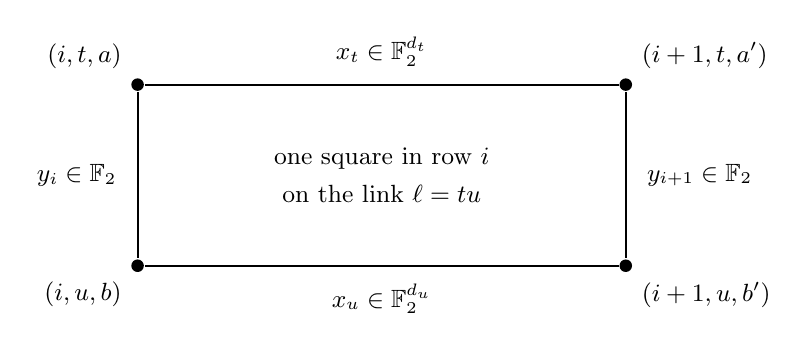
\begin{tikzpicture}[x=1cm,y=1cm,line width=.7pt,font=\small]
 \node[circle,fill,inner sep=1.6pt] (tl) at (0,0) {};
 \node[circle,fill,inner sep=1.6pt] (tr) at (6.2,0) {};
 \node[circle,fill,inner sep=1.6pt] (bl) at (0,-2.3) {};
 \node[circle,fill,inner sep=1.6pt] (br) at (6.2,-2.3) {};
 \draw (tl) -- node[above=3pt] {\(x_t\in\F^{d_t}\)} (tr);
 \draw (bl) -- node[below=3pt] {\(x_u\in\F^{d_u}\)} (br);
 \draw (tl) -- node[left=4pt] {\(y_i\in\F\)} (bl);
 \draw (tr) -- node[right=4pt] {\(y_{i+1}\in\F\)} (br);
 \node[above left=3pt] at (tl) {\((i,t,a)\)};
 \node[above right=3pt] at (tr) {\((i+1,t,a')\)};
 \node[below left=3pt] at (bl) {\((i,u,b)\)};
 \node[below right=3pt] at (br) {\((i+1,u,b')\)};
 \node[align=center] at (3.1,-1.15)
   {one square in row \(i\)\\[3pt]on the link \(\ell=tu\)};
\end{tikzpicture}
\caption{The corner diagram of a single square. The side labels satisfy
\((a,b)\in\cM_{\ell,i}\) and
\((a',b')\in\cM_{\ell,i+1}\). The horizontal readouts are vector-valued;
the vertical readouts are scalar.
These corners belong to the affine data; the output-graph vertices are
introduced in the next section.}
\label{offset:fig-square}
\end{figure}


\subsection{The extension target and a site-ring model}

The block translations needed in the game must preserve every offset
already chosen, while permitting one more block to be added. The following
statement gives that extension property together with closure under
discarding blocks. Its proof occupies the rest of this section.

\begin{proposition}[Compatible offsets with exact projection]
\label{prop:exact-projection}
If the product scalar-image instance is consistent, there are nonempty
families \(\cH_U\), for every \(U\subseteq\cB\) with \(\abs{U}\le K\),
of lists
\[
  \boldsymbol\xi=(\xi_B)_{B\in U},\qquad \xi_B\in\cZ_B^1,
\]
such that the offsets within a list agree on every shared readout and
\begin{equation}
       \cH_U|_V=\cH_V
       \qquad\text{whenever }V\subseteq U.
       \label{eq:exact-projection}
\end{equation}
Here restriction deletes the entries belonging to \(U\setminus V\).
\end{proposition}

The families select suitable compatible lists; every list in a smaller
family must extend to each permitted larger block set.

A ring of sites illustrates how closing a cycle can constrain a shift
in this extension problem. Fix a type \(t\) and an allowed address
\(\mathbf a\in\prod_{i=1}^r A_{t,i}\). The \(r\) site blocks with
readouts \(x_i=x_{i,t,a_i,a_{i+1}}\) form a cycle on the corners
\((i,t,a_i)\). For this model, choose vectors
\(M_1,\ldots,M_r,h\in\F^{d_t}\), set \(M_{r+1}=M_1\), and write
\[
             x_i=M_i+M_{i+1}+\delta_i h.
\]
Every potential \(M_i\) occurs twice in the ring sum. Since only
\(\delta_r\) is nonzero,
\[
                         \sum_{i=1}^r x_i=h.
\]
Thus the complete ring determines the shift \(h\). Conversely, if
this equality holds, choosing \(M_1\) and solving successively around
the cycle gives potentials realizing all the \(x_i\).

After one site is deleted, the retained edges form a path. For any
new shift \(\widetilde h\), its potentials can be solved successively
along that path while all retained \(x_i\) stay fixed. The missing
edge removes the ring-sum constraint. Put \(g=\widetilde h+h\).
Figure~\ref{fig:projection-gauge} shows one such adjustment.
The general proof must handle squares,
partial address domains, and several components that merge when a
block is added. The next two lemmas generalize the cycle distinction:
a closed walk that crosses the row-\(r\) seam an odd number of times
needs at least \(r\) blocks, and with exactly \(r\) it determines a
full address. On components without such a walk, a later potential
adjustment preserves all retained readouts.

\begin{figure}[tbp]
\centering
\begin{minipage}[t]{0.47\linewidth}
\centering
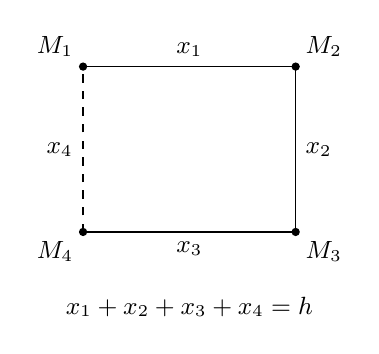
\begin{tikzpicture}[font=\small,line width=0.5pt]
 \coordinate (v1) at (0,0);
 \coordinate (v2) at (2.7,0);
 \coordinate (v3) at (2.7,-2.1);
 \coordinate (v4) at (0,-2.1);
 \draw (v1)--node[above]{$x_1$}(v2)
       --node[right]{$x_2$}(v3)
       --node[below]{$x_3$}(v4);
 \draw[dashed,thick] (v4)--node[left]{$x_4$}(v1);
 \foreach \v in {v1,v2,v3,v4} \fill (\v) circle (1.5pt);
 \node[above left] at (v1) {$M_1$};
 \node[above right] at (v2) {$M_2$};
 \node[below right] at (v3) {$M_3$};
 \node[below left] at (v4) {$M_4$};
 \node at (1.35,-3.05) {$x_1+x_2+x_3+x_4=h$};
\end{tikzpicture}
\end{minipage}\hfill
\begin{minipage}[t]{0.50\linewidth}
\centering
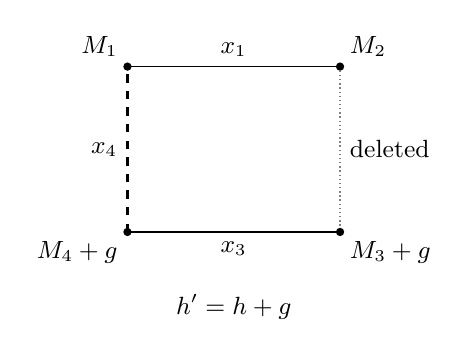
\begin{tikzpicture}[font=\small,line width=0.5pt]
 \coordinate (v1) at (0,0);
 \coordinate (v2) at (2.7,0);
 \coordinate (v3) at (2.7,-2.1);
 \coordinate (v4) at (0,-2.1);
 \draw (v1)--node[above]{$x_1$}(v2);
 \draw[densely dotted,gray] (v2)--node[right,text=black]{deleted}(v3);
 \draw (v3)--node[below]{$x_3$}(v4);
 \draw[dashed,thick] (v4)--node[left]{$x_4$}(v1);
 \foreach \v in {v1,v2,v3,v4} \fill (\v) circle (1.5pt);
 \node[above left] at (v1) {$M_1$};
 \node[above right] at (v2) {$M_2$};
 \node[below right] at (v3) {$M_3+g$};
 \node[below left] at (v4) {$M_4+g$};
 \node[align=center] at (1.35,-3.05)
   {$h'=h+g$};
\end{tikzpicture}
\end{minipage}
\caption{A site ring and the potential adjustment at one type and
one address, with $r=4$.  The dashed edge is the row-$4$ seam.
Left: every potential occurs twice in the sum, leaving $h$.
Right: after deleting row $2$, changing $h$ to $h+g$ and adding $g$
to $M_3,M_4$ preserves every retained readout.  The dotted segment
is absent from the retained corner graph.  The general proof uses
\Cref{offset:lem-gauge} on any nonwrapping component,
not only a cut site ring.}
\label{fig:projection-gauge}
\end{figure}


\subsection{Small supports and recovered addresses}
\label{offset:small-supports}

For \(U\subseteq\cB\), let \(\Gamma_U\) be the union of the corner
diagrams of its blocks. Shared corners and shared named edges are
identified. A block belongs wholly to one connected component of
\(\Gamma_U\). The \emph{support} of a component is its set of types and
its set of distinct wire links: horizontals stay at one type, whereas
verticals project to their links. In particular, several squares on the
same link do not create several support edges.
Write \(\mathcal T(C)\) for the set of types in the support of \(C\).

\begin{lemma}[Small supports]
\label{offset:lem-support}
If \(\abs{U}\le K\), the support of every component of \(\Gamma_U\) is a
tree with at most one real type. Without a real type, it lies in the
interior of a single wire. With a real type, it consists of that type
and possibly initial arms of wires incident with it.
\end{lemma}

\begin{proof}
The support is connected because the corner component is connected.
Only square blocks introduce support links, so it has at most
\(\abs{U}\le K\) distinct links. Internal wire types are private and have
degree two in the full wire layout. A path connecting distinct real
types, or a cycle in that layout, must therefore contain a whole wire,
which has \(4K+1>K\) links. Neither can occur in this support.
This also excludes a cycle created by a loop schema or by parallel
schemas. The stated descriptions follow by following the private wire
interiors from the unique real type, if one is present.
\end{proof}

For every coordinate of every oriented link, fix a permutation
\(\pi_{\ell,i}\) of the ambient label set \(\{0,1\}\) that extends its
matches. Such a permutation exists because those matches are the graph
of an injection on a nonempty binary subset. Use the identity for
identity matches, including partial identities, and use
\(\pi_{\ell,i}^{-1}\) in the reverse direction. These permutations are
analytical choices; actual vertical edges still use only actual matches.

In a support tree, fix a reference type. Unique paths transport the
ambient labels at each type to the reference, separately at each
coordinate. We call the transported labels \emph{aligned labels}.
Every vertical edge preserves its aligned label. Changing the reference
applies the same coordinate permutation to all labels, and restricting
to a subtree gives the same alignment up to this change of reference.
Consequently an aligned binary address can be expressed at any type in
the support. Its expression at an internal type need not satisfy that
wire's full address domain unless a further argument supplies this fact.

Assign a marker \(\omega\in\F\) to each named edge: a horizontal in row
\(i\) has marker \(\delta_i\), and a vertical has marker zero.
A collection of blocks, or a corner component, is \emph{wrapping} if its
diagram contains a closed walk whose marker sum is one. Traversals,
including repeated traversals, are counted in this sum.

\begin{lemma}[Wrapping and address recovery]
\label{offset:lem-wrapping}
Let \(\abs{U}\le r+1\).
\begin{enumerate}
 \item Every wrapping subcollection of \(U\) has at least \(r\) blocks.
 \item A wrapping subcollection with exactly \(r\) blocks has one block
 in each row, lies in a single corner component, and determines a unique
 full aligned address.
 \item Any two wrapping \(r\)-block subcollections of \(U\) lie in the
 same corner component and determine the same address in that
 component's alignment.
 \item If the support of a wrapping \(r\)-block subcollection has no real
 type, it lies in a single wire \(e\), and its recovered address,
 expressed in that wire's internal labels, belongs to \(A_e\).
\end{enumerate}
\end{lemma}

\begin{proof}
Take a marker-one closed walk. Let \(c_i\in\F\) be the parity of its
horizontal traversals in row \(i\). Counting incidences at all corners
on boundary \(i\) gives
\[
 c_{i-1}+c_i=0.
\]
Indeed, the total incidence count of a closed walk at those corners is
even, and a vertical traversal contributes twice on the same boundary.
Since the marker sum is \(c_r=1\), all \(c_i\) equal one. Each row
therefore contributes a horizontal edge to the walk, and every block
has horizontals in just one row. This proves the first assertion.

With exactly \(r\) blocks, there must be one block in every row.
The witness walk meets all of them, so all lie in its corner component.
Use the alignment of that component, or of any containing corner
component in \(\Gamma_U\). The horizontals of the unique row-\(i\)
block prescribe one aligned label at boundary \(i\) and one at boundary
\(i+1\): for a square the two horizontals have the same aligned labels
because of its vertical matches.

Now count incidences at boundary \(i\) separately for each aligned label.
Vertical traversals contribute an even number of incidences to that
label. The total horizontal contribution from each neighboring row is
odd and occurs at that row's prescribed label. The labels prescribed
by rows \(i-1\) and \(i\) must therefore agree. Their common value is the
\(i\)-th coordinate of the recovered address. This proves existence and
uniqueness.

Two \(r\)-element subcollections of a set of size at most \(r+1\) share
at least \(r-1\) blocks. In the present setting these common blocks have
distinct rows. In particular, the two subcollections are in the same
corner component. Every boundary is incident with a common row, since
at most one row is missing from the overlap and \(r\ge3\). Its address
coordinate is consequently the same for both subcollections.

Finally, a support without a real type is inside one wire by
\Cref{offset:lem-support}. All its internal matches are identities.
Every recovered coordinate is the label of a corner at an internal
type, and hence lies in \(A_{e,i}\). Reading all coordinates gives an
address in \(A_e\).
\end{proof}

Only wrapping subcollections of exactly \(r\) blocks will select an
address in the construction below. A component with \(r+1\) blocks may
wrap without containing such a subcollection; no address condition will
be imposed on that component.

\subsection{Admissible shifts and corner potentials}
\label{offset:shifts}

Suppose now that the scalar-image instance is consistent, and fix
nonempty witnesses \(Q_{P,\mathbf a}\) satisfying
\Cref{eq:scalar-images}. For every wire \(e:P\to R\) and every
\(\mathbf a\in A_e\), define the nonempty scalar set
\begin{equation}
 D_{e,\mathbf a}
   =\phi_{e,0}(Q_{P,\mathbf a})
   =\phi_{e,1}
       (Q_{R,\boldsymbol\sigma_e(\mathbf a)}).
 \label{offset:eq-wire-images}
\end{equation}
These are individual image equalities, with no requirement on joint
images of different forms.

Fix \(U\subseteq\cB\) with \(\abs{U}\le K\), and a component \(C\) of
\(\Gamma_U\). A \emph{shift system} on \(C\) is a vector
\[
 (h_t)_{t\in\mathcal T(C)},\qquad h_t\in\F^{d_t},
\]
satisfying \Cref{eq:link-equation} on every support link. Its coordinates
are indexed by the types of this component: different corner components
may use different shifts at the same type.

We call the shift system \emph{admissible} if it also satisfies the
following condition whenever \(C\) contains a wrapping \(r\)-block
subcollection. By \Cref{offset:lem-wrapping}, the recovered address is
independent of that subcollection.
\begin{itemize}
 \item If the support contains a real type \(P\), express the recovered
 address there as \(\mathbf a_P\), and require
 \(h_P\in Q_{P,\mathbf a_P}\).
 \item If the support has no real type, let \(e\) be its wire, express the
 recovered address in the internal labels as \(\mathbf a\), and require
 the common internal scalar to belong to \(D_{e,\mathbf a}\).
 The address lies in \(A_e\) by \Cref{offset:lem-wrapping}.
\end{itemize}
If \(C\) contains no wrapping \(r\)-block subcollection, there is no
additional condition. Write \(\mathcal S(C)\) for the set of admissible
shift systems.

\begin{lemma}[Existence of shifts]
\label{offset:lem-shifts-exist}
Every set \(\mathcal S(C)\) just defined is nonempty.
\end{lemma}

\begin{proof}
If the support has no real type, all its types lie in one wire interior.
Its equations merely identify their scalar shifts. Choose any scalar,
or any element of \(D_{e,\mathbf a}\) when that condition is present.
If the support has a real type \(P\), choose any vector in
\(\F^{d_P}\), or any vector of \(Q_{P,\mathbf a_P}\) when required.
The endpoint equation then determines the scalar along each incident
arm, and the interior equations propagate it along that arm. The arms
do not meet, so there is no further compatibility requirement.
\end{proof}

In particular, when a real type is present we do not additionally impose
an image-set condition on every arm. Some arm may not admit the
recovered address in its full wire domain. Its shift is nevertheless
well defined by the endpoint equation, which is the only condition
needed there.

Choose independently an admissible shift system on each corner
component. At every corner \(v=(i,t,a)\), choose an arbitrary potential
\(M_v\in\F^{d_t}\). Define values on its component's named edges by
\begin{equation}
\begin{aligned}
 x_{vw}&=M_v+M_w+\delta_i h_t
 &&\text{for a horizontal in row \(i\) at type \(t\)},\\
 y_{vw}&=L_{\ell,t}M_v+L_{\ell,u}M_w
 &&\text{for a vertical on \(\ell=tu\)}.
\end{aligned}
\label{offset:eq-potentials}
\end{equation}
Every square satisfies \Cref{eq:square-equation} with \(\eps=1\).
Indeed, each corner potential occurs twice in its boundary expression
and cancels, leaving
\[
 \delta_i\bigl(L_{\ell,t}h_t+L_{\ell,u}h_u\bigr)
       =\delta_i b_\ell.
\]
Sites have no equation. Since a named edge is assigned only one value,
the resulting offsets agree on all readouts shared between blocks.

Define \(\cH_U\) to be the set of all lists
\[
  \boldsymbol\xi=(\xi_B)_{B\in U},
  \qquad \xi_B\in\cZ_B^1,
\]
obtained in this way from admissible shifts and arbitrary corner
potentials. The shifts exist by \Cref{offset:lem-shifts-exist}, so
\(\cH_U\) is nonempty. For \(U=\varnothing\), it consists of the empty
list. We make no uniqueness claim for representations by shifts and
potentials; all permitted representations contribute to the same family.

\subsection{Restriction and extension}
\label{offset:restriction}

Two lemmas isolate the roles of wrapping and nonwrapping components.
The first concerns the shifts themselves, whereas the second permits
shifts to change while preserving the represented offsets.

\begin{lemma}[Lifting shifts from a wrapping component]
\label{offset:lem-wrapping-lift}
Let \(V\subsetneq U\subseteq\cB\), with \(\abs{U}\le r+1\).
If \(C_0\) is a wrapping component of \(\Gamma_V\), and \(C\) is its
containing component in \(\Gamma_U\), restriction of shift systems defines
a surjection
\[
    \mathcal S(C)\longrightarrow\mathcal S(C_0).
\]
\end{lemma}

\begin{proof}
We have \(\abs{V}\le r\). By \Cref{offset:lem-wrapping}, \(C_0\) uses
exactly \(r\) blocks. Its recovered address is the one used for \(C\),
expressed in the respective coordinate systems. There are three cases.

If the support of \(C_0\) contains a real type \(P\), it is also the
unique real type of \(C\). The admissible systems on either component
are parameterized by the same vector \(h_P\in Q_{P,\mathbf a_P}\);
that vector determines the scalars on all of their arms. Restriction
preserves this parameter and is onto.

If the support of \(C\) has no real type, both components are inside the
same wire \(e\). Their admissible systems are parameterized by the same
scalar in \(D_{e,\mathbf a}\), so restriction is again onto.

In the remaining case, \(C\) contains a real type \(P\), but \(C_0\) does
not. The connected support of \(C_0\) lies inside one arm at \(P\),
belonging to a wire \(e\). Its recovered internal address
\(\mathbf a\) belongs to \(A_e\). Therefore the ambient permutation
transport from that address to the incident real endpoint agrees, on
every coordinate, with the actual endpoint map: it is the identity if
\(P\) is the first endpoint, and \(\boldsymbol\sigma_e\) if \(P\) is the
second. Thus the map from the parameter for \(C\) to the parameter for
\(C_0\) is respectively
\[
 \phi_{e,0}:Q_{P,\mathbf a}\longrightarrow D_{e,\mathbf a},
 \qquad\text{or}\qquad
 \phi_{e,1}:Q_{P,\boldsymbol\sigma_e(\mathbf a)}
                    \longrightarrow D_{e,\mathbf a}.
\]
The applicable map is onto by \Cref{offset:eq-wire-images}.
Once its preimage has been chosen, all the other arm scalars of \(C\)
are determined and admissible. Only the incident endpoint of this arm
is used, so the argument also covers a loop wire. Injectivity of the
endpoint form is not required.
\end{proof}

\begin{lemma}[Changing shifts on a nonwrapping component]
\label{offset:lem-gauge}
Let \(C_0\) be a nonwrapping corner component. Suppose two shift systems
\((h_t)\) and \((\widetilde h_t)\) satisfy the link equations on its
support. Every collection of offsets represented by the first system
and corner potentials can also be represented by the second system
after changing those potentials.
\end{lemma}

\begin{proof}
Put \(g_t=\widetilde h_t+h_t\). Adding the two copies of the link
equation gives
\begin{equation}
   L_{\ell,t}g_t=L_{\ell,u}g_u
   \quad\text{on every support link }\ell=tu.
   \label{offset:eq-shift-difference}
\end{equation}
Since \(C_0\) is nonwrapping, the marker sum is zero on every closed walk.
Choose one corner as a root, and define \(s_v\in\F\) to be the marker sum
along a path from it to \(v\). This is independent of the path: the
concatenation of two such paths, reversing one, is a closed walk.
Consequently
\[
     s_v+s_w=\omega(vw)
\]
on every named edge.

Replace the old potential at a corner of type \(t\) by
\(\widetilde M_v=M_v+s_vg_t\). On a horizontal in row \(i\), the change
in \Cref{offset:eq-potentials} is
\[
 (s_v+s_w)g_t+\delta_i(\widetilde h_t+h_t)
       =(\delta_i+\delta_i)g_t=0.
\]
On a vertical, \(s_v=s_w\), so the change is
\[
 s_vL_{\ell,t}g_t+s_wL_{\ell,u}g_u=0
\]
by \Cref{offset:eq-shift-difference}. Thus all old readout values are
preserved. The argument allows vector shifts at a two-dimensional
real type and does not require its endpoint forms to be nonzero.
\end{proof}

\begin{proof}[Proof of \Cref{prop:exact-projection}]
Use the families defined by \Cref{offset:eq-potentials}. Nonemptiness,
legality, and agreement on shared readouts have already been proved.
It remains to establish the projection equality. The case \(V=U\)
is immediate, so suppose \(V\subsetneq U\). Then \(\abs{V}\le r\).
Each component \(C_0\) of \(\Gamma_V\) lies in a component \(C\) of
\(\Gamma_U\).

First take a represented list in \(\cH_U\) and restrict its shifts and
potentials to each \(C_0\). These shifts satisfy all old link equations.
If \(C_0\) is nonwrapping, it has no additional address condition.
If it wraps, their admissibility follows from
\Cref{offset:lem-wrapping-lift}. The restricted representation therefore
belongs to \(\cH_V\), proving
\(\cH_U|_V\subseteq\cH_V\).

For the other inclusion, fix an arbitrary list in \(\cH_V\), and choose
any one of its representations by admissible old shifts and potentials.
There is at most one wrapping old component: one would already require
\(r\) of the at most \(r\) old blocks.
For each component \(C\) of \(\Gamma_U\), choose an admissible new shift
system. If \(C\) contains the wrapping old component \(C_0\), choose it
to extend the selected old shifts on \(C_0\), using
\Cref{offset:lem-wrapping-lift}. On all other new components choose any
admissible shifts.

Keep the old potentials on a wrapping old component. On every
nonwrapping old component, apply \Cref{offset:lem-gauge} to replace its
old shifts by the restriction of the chosen new shifts without changing
any old offset. Distinct old components have disjoint corner sets,
so these potential changes coexist even when several old components
merge into a single new component or have different old shifts at the
same type. Assign arbitrary potentials to the additional corners of
\(\Gamma_U\).

The new shifts and these potentials represent a member of \(\cH_U\).
They satisfy every new square equation by
\Cref{offset:eq-potentials}, while on each old named edge the value is
unchanged. Hence this member restricts to the prescribed list in
\(\cH_V\), proving the reverse inclusion.
\end{proof}

There are two useful features of this proof. First, if a component
first becomes wrapping only when all \(r+1\) blocks are present, it has
no wrapping proper subcollection and no address condition is needed:
all the old components are covered by the gauge lemma. Second, a
wrapping old component asks for at most one scalar preimage from a
real-type witness set. Thus the individual image equalities in
\Cref{offset:eq-wire-images} suffice, even for non-affine witness sets
or noninjective endpoint forms. The families \(\cH_U\), their shifts,
and the witnesses \(Q_{P,\mathbf a}\) are used only in this existence
argument; the reduction never enumerates them.

\section{The general graph realization}\label{general:section}

The blocks of \Cref{offset:section} have two realizations. We first use
one vertex per legal valuation and attach private leaves to identify
its block. This construction has no degree restriction, but gives the
smaller quantitative compiler. Throughout this section \(r\ge3\).
\Cref{reduction:section} proves the game-transfer argument for this
realization. We then construct subcubic graphs with the same affine block
data in \Cref{graph:section}.

\subsection{Valuation vertices and private leaves}

For \(\eps\in\{0,1\}\), create a base vertex \((B,z)\) for every
block \(B\in\cB\) and valuation \(z\in\cZ_B^\eps\). Two base vertices
are adjacent exactly when
\begin{equation}\label{general:adjacency}
 B\ne C,\qquad
 \cR(B)\cap\cR(C)\ne\varnothing,\qquad
 z(\rho)=w(\rho)\quad
 \text{for every }\rho\in\cR(B)\cap\cR(C).
\end{equation}
There are no edges within a block. Agreement is required on
\emph{all} common readouts; disagreement on even one gives a nonedge.

Write \(J=\abs{\cB}\), and let \(N\) be the common number of base
vertices. The base-vertex counts in the two versions agree by
\Cref{lem:block-fibers}.
Number the blocks by \(j(B)\in\{1,\ldots,J\}\) in the same order
in both versions. At each \((B,z)\), attach \(j(B)(N+1)\) private
leaves, adjacent only to that owner. Denote them by
\(\operatorname{leaf}(B,z,\nu)\), where
\(1\le\nu\le j(B)(N+1)\). Call the resulting graphs \(G^0,G^1\),
and let \(V_B^\eps\) contain all base vertices of block \(B\) and
all their leaves. These parts partition the graph.

\begin{proposition}[General realization]\label{prop:general-realization}
For the affine block data at address length \(r\ge3\), the graphs
\(G^0,G^1\) are simple, uncolored, and of the same positive order.
They have \(O(J^3)\) vertices.

Every \(\xi_B\in\cZ_B^1\) determines a fixed bijection
\(\Psi_{B,\xi_B}:V_B^0\to V_B^1\), depending only on \(B,\xi_B\),
by
\[
 (B,z)\longmapsto(B,z+\xi_B),\qquad
 \operatorname{leaf}(B,z,\nu)\longmapsto
 \operatorname{leaf}(B,z+\xi_B,\nu).
\]
For any set \(U\) of blocks, offsets agreeing on all shared readouts
make the union of these maps an isomorphism of the induced subgraphs
on the corresponding parts.

At every history reached by a winning \(K=r+1\)-slot strategy,
a marked base vertex \((B,z)\) is answered by \((B,z')\) with
\(z'\in\cZ_B^1\). If zero base vertices of distinct blocks are
simultaneously marked, their responses agree on every shared
readout, even when all \(K\) slots are occupied.
\end{proposition}

\begin{proof}
The adjacency rule and owner rule introduce no loops or multiple
edges. Each block has nonempty legal fibers of equal cardinality,
so the two graphs have equal positive orders. Each block has at
most \(64\) valuations, a convenient loose constant, hence
\(J\le N\le64J\). The total order is at most
\[
       N+NJ(N+1)=O(J^3).
\]

Translation by a legal affine offset bijects \(\cZ_B^0\) with
\(\cZ_B^1\). All owners in block \(B\) have the same number of
leaves, so the displayed map is a bijection of the entire part.
Within a base block it preserves equality, and there are no base
edges. Between distinct active blocks the offsets agree on every
shared readout; adding equal offsets preserves both agreement and
disagreement on each name, hence the entire condition
\eqref{general:adjacency}. Blocks with no common name stay
nonadjacent.

A leaf is adjacent only to its owner. For a base vertex in the
owner's block the same translation is applied to the base and the
owner, whether or not the owner itself is marked, so their equality
is preserved. A base in a different block remains a nonowner.
Distinct leaves stay distinct because owner translation is
injective and the local index is unchanged. Repeated selections,
different leaves at one owner, and leaves at different owners are
therefore all handled. Leaf--leaf adjacency is absent, and no leaf
is identified with a base vertex. This proves the induced-subgraph
claim on any union of compatible parts.

For recognition, first observe that a marked pair reached under
any winning strategy with at least two slots has equal degrees.
After discarding every other pair, request another slot. The
announced bijection must preserve adjacency to the retained pair
for every choice, and therefore matches its two neighborhoods
bijectively. This is a property of the reached history, not a test
that needs spare slots in that history.

Every leaf has degree one. A base vertex in block number \(j\)
has degree in
\[
       [j(N+1),\,j(N+1)+N-1].
\]
These intervals are disjoint and have lower endpoints greater
than one. Thus every reached base response is a legal valuation
in the same block. Distinct homogeneous zero vertices sharing
a readout are adjacent, so their responses must satisfy
\eqref{general:adjacency} and agree on all shared names.
\end{proof}

The proposition supplies both interfaces needed for the game:
compatible offsets induce blockwise maps on \emph{all} vertices,
including leaves, while zero queries decode to legal affine
valuations with shared-readout agreement. The ring-transfer proof
in \Cref{reduction:section} will use only those interfaces.

\section{From block realizations to the bijective game}
\label{reduction:section}

The general graph construction has two properties with different roles.
Compatible offsets act by bijections on entire block parts, which will
supply Duplicator's announced map. Conversely, a marked zero valuation
receives a legal affine valuation, and simultaneous zero responses agree
on shared readouts. These responses will recover the witness sets of
the scalar-image instance.

We now prove that these two properties suffice. Stating their precise
form here lets the subcubic construction in \Cref{graph:section} use
the same argument after verifying the same conditions. The present
proof uses only the affine blocks of \Cref{offset:section}; it does
not require the later construction.

\begin{proposition}[A realization interface for the game]
\label{prop:game-reduction}
Let a product scalar-image instance have address length \(r\ge3\),
put \(K=r+1\), and form its affine block data. Suppose finite simple
graphs \(W^0,W^1\) of the same positive order have partitions
\[
 V(W^\eps)=\coprod_{B\in\cB}V_B^\eps
 \qquad(\eps\in\{0,1\})
\]
with the following properties.
\begin{enumerate}
\item\label{item:game-local-maps}
For every block \(B\) and offset \(\xi_B\in\cZ_B^1\), there is a
fixed bijection
\(\Psi_{B,\xi_B}:V_B^0\to V_B^1\), depending only on that offset
and the constructed graphs. Whenever offsets on a set of blocks agree
on shared readouts, the union of their maps is an isomorphism of the
induced subgraphs on the corresponding parts.
\item\label{item:game-zero-decoding}
For every \(B\), \(\eps\), and \(z\in\cZ_B^\eps\), there is a
nonempty set \(\mathcal D_B^\eps(z)\subseteq V_B^\eps\); for fixed
\(B,\eps\), these sets are pairwise disjoint. At every history
reached under any winning \(K\)-slot strategy, a marked vertex in
\(\mathcal D_B^0(0)\) is answered by a vertex in
\(\mathcal D_B^1(\zeta_B)\) for some \(\zeta_B\in\cZ_B^1\).
For simultaneous such marks in distinct blocks \(B,C\), the decoded
valuations \(\zeta_B,\zeta_C\) agree on every shared readout.
These assertions apply also when all slots are occupied.
\end{enumerate}
Then
\[
 \text{the instance is consistent}
 \quad\Longleftrightarrow\quad
 \text{Duplicator wins on \(W^0,W^1\) with \(K\) slots}
 \quad\Longleftrightarrow\quad W^0\equiv_r W^1.
\]
\end{proposition}

For the general construction, the query sets are simply
\(\mathcal D_B^\eps(z)=\{(B,z)\}\), and both hypotheses follow from
\Cref{prop:general-realization}. The sets \(\mathcal D_B^\eps(z)\)
allow one valuation to have several query vertices. This flexibility
will let the subcubic construction use a triangle for each valuation.

\begin{proof}
\Cref{lem:wl-game} gives the game/WL equivalence because \(r\ge3\).
We prove the two directions involving consistency from the stated
realization properties.

\paragraph{Witness sets give a winning strategy.}
Suppose the instance has witnesses, and take the nonempty families
$\cH_U$ supplied by \Cref{prop:exact-projection} for every set of blocks
$U$ with $\abs{U}\leq K$.  Recall that their restriction maps satisfy
\eqref{eq:exact-projection} and that every list in such a family agrees on
all shared readouts.

Call a block \emph{active} when its part $V_B^0$ contains a currently
marked first-graph vertex.  Duplicator maintains the following invariant:
if $U$ is the active set, there is a list
\[
 \boldsymbol\xi=(\xi_B)_{B\in U}\in\cH_U
\]
such that every marked vertex $v\in V_B^0$ is paired with
$\Psi_{B,\xi_B}(v)$.  By the local-map hypothesis, the union of these maps is an isomorphism
between the induced subgraphs on the active parts.  In particular, the marked pairs form a partial isomorphism.
Initially $U=\varnothing$, and the invariant holds with the empty list.
After any discards, restrict the list to the remaining active set; exact
projection, in particular its restriction inclusion, keeps it in the
required family.

Suppose a vacant slot is requested.  There are at most $K-1=r$ occupied
slots, so $\abs{U}\leq r$.  For \emph{each} inactive block $B$, choose a
list
\begin{equation}
\label{uniform:preselected-extension}
 \boldsymbol\eta^{\,B}\in\cH_{U\cup\{B\}},
 \qquad
 \boldsymbol\eta^{\,B}|_U=\boldsymbol\xi.
\end{equation}
Such a list exists by the extension direction of exact projection.
All of these choices are made before Spoiler's vertex choice.  They may,
for example, be made using fixed orders on the finite sets of possible
offset lists.  Define a map on the whole first graph by
\[
 f|_{V_B^0}=
 \begin{cases}
  \Psi_{B,\xi_B},&B\in U,\\
  \Psi_{B,\eta^{\,B}_B},&B\notin U.
 \end{cases}
\]
Every piece is a bijection from $V_B^0$ onto $V_B^1$, and these parts
partition the two vertex sets.  Hence $f$ is one bijection of the entire
graphs, which Duplicator announces.

If Spoiler chooses a vertex in an active block, retain the current list.
Otherwise, if the chosen vertex lies in $V_B^0$, use the particular list
$\boldsymbol\eta^{\,B}$ from~\eqref{uniform:preselected-extension} as the
new invariant.  It agrees with every old active-block offset and gives the
announced image of the newly chosen vertex.  No second inactive block
becomes active during this move.  Thus compatibility between the choices
made for two different inactive blocks is unnecessary: only one of those
choices is used to update the invariant.  This proves that Duplicator wins
through every finite history.

\paragraph{A winning strategy gives attained image sets.}
Fix a winning strategy.  For each block \(B\), choose once and for all a
vertex \(z_B\in\mathcal D_B^0(0)\) representing its zero valuation.
This set is nonempty because \(0\in\cZ_B^0\).  A
\emph{zero-query history} is a finite history from empty under the fixed
strategy in which every vertex chosen by Spoiler is one of these $z_B$;
discards are unrestricted.

By the zero-decoding hypothesis, a response to \(z_B\) lies in
\(\mathcal D_B^1(\zeta_B)\) for a uniquely determined legal valuation
$\zeta_B\in\cZ_B^1$.  If zero representatives of distinct blocks are
simultaneously marked, their response valuations agree on every shared
readout. This is the second realization hypothesis, applied at the
current history even when all $K$ slots are occupied. No further test
needs to be executed during a zero-query history. Once a pair is marked,
its actual response vertex and its decoded valuation remain fixed until
that pair is discarded.

For a type $t$ and an allowed full address
$\mathbf a\in\prod_{i=1}^r A_{t,i}$, let
$S_i(t,\mathbf a)$ be the site block with readout
$x_{i,t,a_i,a_{i+1}}$, where indices are cyclic.  These $r$ blocks are
distinct because they have distinct row indices.  We call them the
\emph{site ring} at $(t,\mathbf a)$.  At a zero-query history having
precisely one representative of each of these sites marked, define its
ring sum to be
\begin{equation}
\label{uniform:ring-sum}
 h_t=\sum_{i=1}^r
 \zeta_{S_i(t,\mathbf a)}(x_{i,t,a_i,a_{i+1}})
 \ \in\F^{d_t}.
\end{equation}
There are exactly $r$ occupied slots at such a history, in any arrangement,
and one slot is vacant.  We may write $h_t(\mathfrak h)$ to make the
dependence on the particular history $\mathfrak h$ explicit.

For a real type $P$ and $\mathbf a\in\{0,1\}^r$, let
$\mathfrak H_{P,\mathbf a}$ be the set of all finite zero-query histories
from empty under the fixed strategy that end with precisely the site ring
at $(P,\mathbf a)$ marked, one pair per site in any arrangement of the
slots.  Define
\begin{equation}
\label{uniform:attained-sets}
 Q_{P,\mathbf a}
 =\{h_P(\mathfrak h):\mathfrak h\in\mathfrak H_{P,\mathbf a}\}
 \subseteq\F^{d_P}.
\end{equation}
The definition ranges over \emph{all} such histories under the one fixed
strategy.  Directly querying the $r$ ring sites from empty shows that
every $Q_{P,\mathbf a}$ is nonempty.  We will verify the individual image
equalities for these sets without requiring the strategy to give the same
response on a later visit to a ring.

\paragraph{Transferring one ring across a link.}
Let $\ell=tu$ be a link.  Fix allowed addresses $\mathbf a$ at $t$ and
$\mathbf b$ at $u$ with
$(a_i,b_i)\in\cM_{\ell,i}$ for every $i$.  For this paragraph write
\[
 T_i=S_i(t,\mathbf a),\qquad U_i=S_i(u,\mathbf b),
\]
and let $B_i$ be the square in row $i$ determined by the matches
$(a_i,b_i)$ and $(a_{i+1},b_{i+1})$.  Its horizontal names are the readouts
of $T_i$ and $U_i$, and its vertical names are
\[
 y_i=y_{i,\ell,a_i,b_i},\qquad
 y_{i+1}=y_{i+1,\ell,a_{i+1},b_{i+1}}.
\]
The two endpoint types of a link are distinct, including on a subdivided
loop schema.  In each of these lists the row blocks are distinct, and sites
are distinct from squares.
\Cref{uniform:fig-ring-transfer} displays the two phases and the role of
the spare slot.

Start at any zero-query history with precisely the $T_i$ marked.  Denote
their decoded horizontal vectors by $\alpha_i$, and fix the numerical
value $h_t=\sum_i\alpha_i$ from this starting history.  For
$i=1,\ldots,r$, place $z_{B_i}$ in the vacant slot \emph{before}
discarding the pair at $T_i$.  During that placement there are $r+1=K$
occupied slots.  Since $B_i$ and $T_i$ are then simultaneously marked and
share their $t$-horizontal, the new square's response has that horizontal
equal to $\alpha_i$.

More explicitly, after processing rows $1,\ldots,j$, the marked blocks are
exactly
\[
 B_1,\ldots,B_j,T_{j+1},\ldots,T_r.
\]
For $i\leq j$, the marked square retains $\alpha_i$ on its
$t$-horizontal.  For $i>j$, the original site pair is still present and
retains $\alpha_i$.  This proves by induction that after the first phase
all $r$ squares are marked and their old-side horizontals are the original
vectors $\alpha_i$, not newly selected ring values.

At this all-square history, write $\beta_i$ for the response's
$u$-horizontal in $B_i$.  The adjacent squares $B_{i-1}$ and $B_i$ share
the name $y_i$, so their values on it agree; denote the common value by
$\eta_i$.  The legal valuation equation
\eqref{eq:square-equation}, in version one, reads
\[
 L_{\ell,t}\alpha_i+L_{\ell,u}\beta_i+\eta_i+\eta_{i+1}
   =\delta_i b_\ell.
\]
Summing over all rows cancels each vertical value twice in $\F$.  Since
$\sum_i\delta_i=1$, this gives
\begin{equation}
\label{uniform:transfer-sum}
 L_{\ell,t}h_t+L_{\ell,u}\sum_{i=1}^r\beta_i=b_\ell.
\end{equation}

\begin{figure}[htbp]
\centering
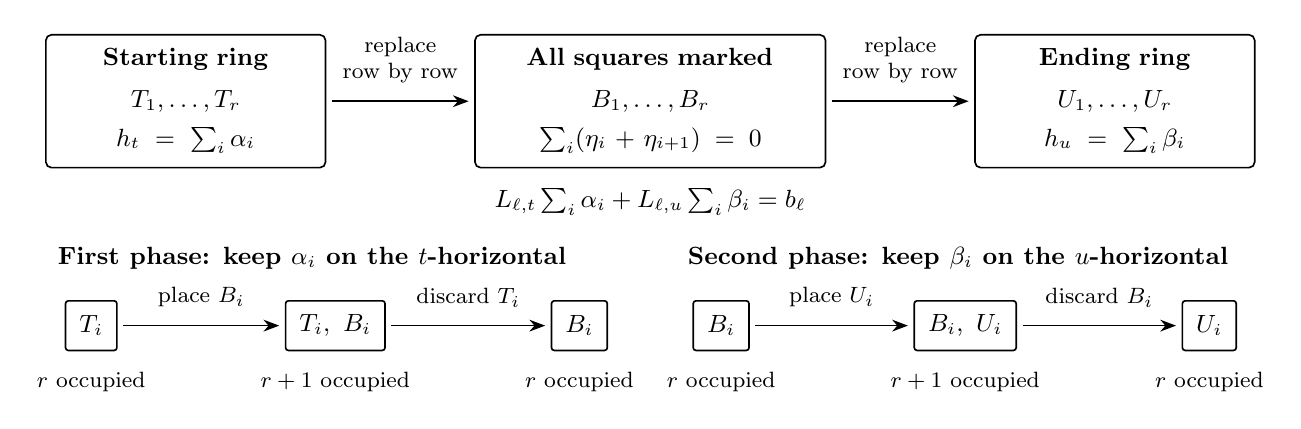
\begin{tikzpicture}[
 x=1cm,y=1cm,line width=.6pt,font=\small,
 stage/.style={draw,rounded corners=2pt,align=center,inner sep=5pt,
               minimum height=1.55cm},
 move/.style={-{Stealth[length=2mm]},shorten >=2pt,shorten <=2pt},
 state/.style={draw,rounded corners=1pt,minimum height=.63cm,
               inner xsep=5pt,align=center}]
 \node[stage,text width=3.2cm] (start) at (1.75,0)
   {\textbf{Starting ring}\\[4pt]
    \(T_1,\ldots,T_r\)\\[3pt]
    \(h_t=\sum_i\alpha_i\)};
 \node[stage,text width=4.1cm] (middle) at (7.65,0)
   {\textbf{All squares marked}\\[4pt]
    \(B_1,\ldots,B_r\)\\[3pt]
    \(\sum_i(\eta_i+\eta_{i+1})=0\)};
 \node[stage,text width=3.2cm] (end) at (13.55,0)
   {\textbf{Ending ring}\\[4pt]
    \(U_1,\ldots,U_r\)\\[3pt]
    \(h_u=\sum_i\beta_i\)};
 \draw[move] (start.east) -- node[above=3pt,align=center,font=\footnotesize]
   {replace\\row by row} (middle.west);
 \draw[move] (middle.east) -- node[above=3pt,align=center,font=\footnotesize]
   {replace\\row by row} (end.west);

 \node[align=center] at (7.65,-1.28)
   {\(L_{\ell,t}\sum_i\alpha_i+
       L_{\ell,u}\sum_i\beta_i=b_\ell\)};

 \node[anchor=west,font=\small\bfseries] at (0,-2.0)
   {First phase: keep \(\alpha_i\) on the \(t\)-horizontal};
 \node[anchor=west,font=\small\bfseries] at (8.0,-2.0)
   {Second phase: keep \(\beta_i\) on the \(u\)-horizontal};
 \node[state] (t) at (.55,-2.85) {\(T_i\)};
 \node[state] (tb) at (3.65,-2.85) {\(T_i,\ B_i\)};
 \node[state] (b) at (6.75,-2.85) {\(B_i\)};
 \draw[move] (t.east) -- node[above=3pt,font=\footnotesize]
   {place \(B_i\)} (tb.west);
 \draw[move] (tb.east) -- node[above=3pt,font=\footnotesize]
   {discard \(T_i\)} (b.west);
 \node[state] (bb) at (8.55,-2.85) {\(B_i\)};
 \node[state] (bu) at (11.65,-2.85) {\(B_i,\ U_i\)};
 \node[state] (u) at (14.75,-2.85) {\(U_i\)};
 \draw[move] (bb.east) -- node[above=3pt,font=\footnotesize]
   {place \(U_i\)} (bu.west);
 \draw[move] (bu.east) -- node[above=3pt,font=\footnotesize]
   {discard \(B_i\)} (u.west);
 \foreach \name/\count in {t/r,tb/{r+1},b/r,bb/r,bu/{r+1},u/r}
   \node[below=4pt,font=\footnotesize] at (\name.south)
     {\(\count\) occupied};
\end{tikzpicture}
\caption{One-link transfer across \(\ell=tu\). Boxes list marked blocks;
arrows are game stages, not output-graph edges. Each row replacement below
keeps the other \(r-1\) marks fixed and places the new zero representative
before discarding the old pair. Simultaneous marks preserve the shared
horizontal value. Each \(B_i\) retains the starting \(t\)-horizontal
\(\alpha_i\). At the common all-square history, \(\beta_i\) is its
\(u\)-horizontal and \(\eta_i\) is the shared value on \(y_i\).
Summing the square equations cancels each \(\eta_i\) twice over \(\F\)
and gives the displayed relation. Each \(U_i\) retains the \(\beta_i\)
from that history. No response must recur after its pair is discarded.}
\label{uniform:fig-ring-transfer}
\end{figure}


Now replace each $B_i$ by $U_i$, again placing the site's zero
representative before removing the square's pair.  The shared
$u$-horizontal copies $\beta_i$ into the new site's response.  After
processing rows $1,\ldots,j$, the marked blocks are
$U_1,\ldots,U_j,B_{j+1},\ldots,B_r$; the new sites retain their copied
$\beta_i$ and the remaining squares retain the values fixed at the
all-square history.  At the end, precisely the $u$-ring is marked and its
sum is $h_u=\sum_i\beta_i$.  Thus the starting and ending sums satisfy
\begin{equation}
\label{uniform:attained-link}
 L_{\ell,t}h_t+L_{\ell,u}h_u=b_\ell.
\end{equation}
Every replacement changes the occupied-slot count from $r$ to $r+1$ and
back to $r$.  The whole transfer uses $2r$ placements and $2r$ discards,
and every chosen vertex is still a fixed zero representative.

This construction also works starting at the $u$-ring: first replace its
sites by the same squares, then replace the squares by the $t$-sites.
The same equation holds with the starting value at $u$ fixed.  No response
is required to recur after its pair has been discarded.

\paragraph{Transferring along a whole comparison wire.}
Fix a schema $e:P\to R$ and an address $\mathbf a\in A_e$.  Along its
wire use $\mathbf a$ at $P$ and at every internal type, and
$\boldsymbol\sigma_e(\mathbf a)$ at $R$.  These are allowed addresses,
and their adjacent coordinates are actual matches at every link: all
but the last link use the restricted identity, while the last uses
$(a_i,\sigma_{e,i}(a_i))$ at coordinate $i$.

Take any $h_P\in Q_{P,\mathbf a}$, choose one witnessing history in
\eqref{uniform:attained-sets}, and continue it by the link transfers just
proved.  The final history is another finite zero-query history, now ending
with exactly the $R,\boldsymbol\sigma_e(\mathbf a)$ ring.  Its sum
$h_R$ therefore belongs to
$Q_{R,\boldsymbol\sigma_e(\mathbf a)}$.  The successive sums satisfy
\eqref{uniform:attained-link}.  Interior link equations equate consecutive
scalar shifts, while the two endpoint equations identify their common
value with the endpoint affine forms.  Consequently,
\[
 \phi_{e,0}(h_P)=\phi_{e,1}(h_R).
\]
This proves
\[
 \phi_{e,0}(Q_{P,\mathbf a})
 \subseteq
 \phi_{e,1}(Q_{R,\boldsymbol\sigma_e(\mathbf a)}).
\]

For the opposite inclusion, start from any history witnessing an element
of $Q_{R,\boldsymbol\sigma_e(\mathbf a)}$ and traverse the wire in reverse.
At its last link, invert each $\sigma_{e,i}$ only on its image: the
specified coordinate $\sigma_{e,i}(a_i)$ has the unique allowed preimage
$a_i$.  All remaining reverse matches are restricted identities.  Thus
the reverse transfer reaches the $P,\mathbf a$ ring and proves the other
inclusion.  No surjectivity of a partial coordinate injection onto the
ambient binary set has been used.

If $P=R$, the endpoint rings are still successive occurrences in the
history.  Their decoded responses may differ, even if the two addresses
are equal.  Both attained values belong to the appropriate set in
\eqref{uniform:attained-sets}, which is all that the image equality requires.
Likewise, separate schemas need no simultaneous choice of endpoint
witnesses.  We have proved \eqref{eq:scalar-images} for every schema and
every address in its domain, establishing consistency.
\end{proof}


\begin{corollary}[Correctness of the general realization]
\label{cor:general-game}
For every product scalar-image instance at address length \(r\ge3\),
its general realization satisfies
\[
 \text{the instance is consistent}\quad\Longleftrightarrow\quad
 G^0\equiv_r G^1.
\]
\end{corollary}
\begin{proof}
Apply \Cref{prop:game-reduction} with the parts, maps and singleton
query sets supplied by \Cref{prop:general-realization}.
\end{proof}

\section{A subcubic realization of the affine blocks}
\label{graph:section}

We now encode the block data by graphs of maximum degree three while
meeting the two hypotheses of \Cref{prop:game-reduction}.
We use the same affine blocks as in the general realization, but replace
the valuation graph and its private leaves by a different graph. Every
new vertex must still belong to just one block, and its local map must
depend only on that block's offset. We prove these properties together
with reached-history recognition; no generic degree-reduction theorem
or unrestricted-degree hardness theorem supplies this step.
Throughout this section take \(r\ge8\), so \(K=r+1\ge9\).

Write \(N=\abs{\cB}\).  We use the following conclusions of
\Cref{lem:block-fibers}.  A block \(B\) has a set \(\cR(B)\) of at most four
readout names, each with its specified one- or two-dimensional binary
value space.  The total number \(a_B\) of scalar coordinates is at most
six.  Its legal valuation sets satisfy
\[
  \cZ_B^0\text{ is a vector space},\qquad
  \cZ_B^1=\cZ_B^0+\xi
       \quad\text{for every }\xi\in\cZ_B^1,
\]
and both sets are nonempty.  Their projections onto any one named
readout are full.  The coordinates of a name have the same prescribed
order at every block that contains that name.  For a valuation \(z\)
and a name \(\rho\in\cR(B)\), write \(z|_\rho\) for its value on that
readout.

\Needspace{5\baselineskip}
\begin{proposition}[Subcubic realization]
\label{prop:subcubic-realization}
From the block data one can construct graphs \(X^0,X^1\), with
partitions
\[
  V(X^\eps)=\coprod_{B\in\cB}V_B^\eps
  \qquad(\eps\in\{0,1\}),
\]
having the following properties.
\begin{enumerate}
\item
Both graphs are finite, simple, connected, uncolored, and of maximum
degree at most three.  They have the same positive order.
Their orders are \(O(N^4)\), and the construction is polynomial in the
size of the explicitly listed block data.
\item
For each \(z\in\cZ_B^\eps\), the part \(V_B^\eps\) contains a specified
triangle \(T_B^\eps(z)\).  These triangles are pairwise disjoint.
For every \(\xi_B\in\cZ_B^1\), there is a fixed bijection
\[
  \Psi_{B,\xi_B}:V_B^0\longrightarrow V_B^1
\]
depending only on \(B,\xi_B\), and the constructed graphs.  It sends
\(T_B^0(z)\) onto \(T_B^1(z+\xi_B)\).
\par\Needspace{7\baselineskip}
If \(U\subseteq\cB\) and the offsets
\((\xi_B)_{B\in U}\) agree on all names shared by blocks in \(U\), then
the following map is an isomorphism of induced subgraphs:
\[
 \coprod_{B\in U}\Psi_{B,\xi_B}:
 X^0\left[\bigcup_{B\in U}V_B^0\right]
 \longrightarrow
 X^1\left[\bigcup_{B\in U}V_B^1\right].
\]
\item
Fix a winning Duplicator strategy in the \(K\)-slot bijection game,
where \(K=r+1\ge9\).
At every reached history, a marked vertex in \(T_B^0(z)\) is paired
with a vertex in \(T_B^1(z')\) for a unique \(z'\in\cZ_B^1\).
If simultaneous marked vertices lie in \(T_B^0(z)\) and \(T_C^0(w)\),
where \(B\ne C\), then, for each
\(\rho\in\cR(B)\cap\cR(C)\),
\[
     z|_\rho=w|_\rho
     \quad\Longrightarrow\quad
     z'|_\rho=w'|_\rho .
\]
These conclusions hold even when all \(K\) slots are occupied.
\end{enumerate}
\end{proposition}

We construct the graphs and establish the proposition in stages.

\subsection{Channels, prefix forests, and a connected colored graph}

For every block \(B\), form an ordered list of \emph{channels}.
Its first member is channel \(0\), which specifies no readout.
For every other block \(C\ne B\) and every shared name
\(\rho\in\cR(B)\cap\cR(C)\), add a channel denoted
\(c_B(C,\rho)\).
The channels \(c_B(C,\rho)\) and \(c_C(B,\rho)\) are called
\emph{opposite}.  Their order is fixed by the block data and is the
same in both versions.

In each channel \(c\) choose an order of the \(a_B\) scalar coordinates,
again common to the two versions.  In a proper channel
\(c=c_B(C,\rho)\), the coordinates of \(\rho\), in their prescribed
order, must come first.  Let
\[
 q_{Bc}=
 \begin{cases}
  0,&c=0,\\
  \dim(\rho),&c=c_B(C,\rho).
 \end{cases}
\]
For a valuation \(z\), denote its length-\(h\) prefix in channel \(c\)'s
order by \(\pi_{Bc,h}(z)\).
We build a vertex-colored graph \(Y^\eps\).
All vertex positions in the following list are distinct.

\begin{enumerate}
\item
\textbf{Spines.}
For every channel \(c\) and legal valuation \(z\in\cZ_B^\eps\),
create a vertex \(s_{Bc}^\eps(z)\).
For consecutive channels \(c,c+1\), join
\(s_{Bc}^\eps(z)\) to \(s_{B,c+1}^\eps(z)\).
Thus each valuation has one path through the channel list.
Set
\[
                  s_B^\eps(z)=s_{B0}^\eps(z)
\]
and call this its distinguished vertex.
\item
\textbf{Prefix forests.}
For \(q_{Bc}\le h\le a_B\), and every prefix \(u\) of length \(h\)
that extends to a valuation in \(\cZ_B^\eps\), create a vertex
\(f_{Bc,h}^\eps(u)\).
For \(h>q_{Bc}\), join it to the vertex indexed by its truncation
to length \(h-1\).
These are rooted trees whose roots have level \(q_{Bc}\).
Join the leaf
\(f_{Bc,a_B}^\eps(\pi_{Bc,a_B}(z))\)
to \(s_{Bc}^\eps(z)\).
\item
\textbf{Anchors.}
Create an anchor \(\alpha_B^\eps\) and join it to
\(f_{B0,0}^\eps(\varnothing)\).
Join the anchors in a path through all blocks in a fixed order.
\item
\textbf{Equality matchings.}
For opposite proper channels specifying \(\rho\), join their roots
with the same value of \(\rho\).
Write \(c=c_B(C,\rho)\), \(c'=c_C(B,\rho)\), and
\(q=\dim(\rho)=q_{Bc}=q_{Cc'}\).
For each \(u\) in the value space of \(\rho\), join
\[
 f_{Bc,q}^\eps(u)
 \quad\text{to}\quad
 f_{Cc',q}^\eps(u).
\]
Full projection onto \(\rho\) ensures that both roots exist for every
\(u\), so this is a perfect matching of the two root sets.
\end{enumerate}

If \(q_{Bc}=a_B\), a root is also a leaf: it is one vertex, adjacent
to its spine vertex and its opposite root.
There is no additional copy or truncation edge in this case.

The \emph{sorts} are: one anchor sort for each block; one spine sort
for each block and channel; and one tree sort for each block, channel,
and level.  If there are \(s\) sorts, assign them the consecutive
integers \(1,\ldots,s\) in a fixed enumeration order, common to the
two versions.
Let \(\operatorname{col}(v)\) be the resulting color of a vertex.
In particular, different labels within a sort receive the same color.
Assign every vertex just constructed at \(B\) to its \emph{block part}.

\begin{lemma}
\label{graph:colored-promises}
Each \(Y^\eps\) is simple, connected, and has maximum degree at most
three.  Each block part is connected.  There are \(O(N^2)\) vertices
and \(O(N^2)\) sorts.
\end{lemma}

\begin{proof}
A spine vertex has at most two spine neighbors and one leaf neighbor.
A nonroot internal tree vertex has one parent and at most two children.
A nonleaf root has at most two children and one further neighbor:
its anchor in channel zero, or its matched opposite root in a proper
channel.  A leaf has its spine neighbor and either its parent or,
when it is also a root, its matched opposite root.
An anchor has its channel-zero root neighbor and at most two neighbors
on the anchor path.
Thus every degree is at most three.

All tree, spine, and anchor vertices occupy distinct positions.
A proper root belongs to just one channel and has just one matching
edge.  Its opposite root belongs to a different block.
The remaining edge types have their distinct indicated endpoints,
so no loop or multiple edge is introduced.

Every legal prefix has a full legal extension.
It therefore reaches a leaf, then the spine at that channel.
The spine path reaches channel zero at the same valuation, and the
channel-zero tree reaches the anchor.
This proves connectedness of each block part.
The anchor path joins all parts.

There are at most
\[
 N+\sum_{B\ne C}\abs{\cR(B)\cap\cR(C)}
 \le N+4N(N-1)
\]
channels in total.
A channel has at most \(2^6\) spine vertices and at most
\(\sum_{h=0}^6 2^h\) tree vertices.
It also has at most eight sorts: one spine sort and at most seven
tree-level sorts.  Adding the \(N\) anchors and anchor sorts proves
both estimates.
\end{proof}

\begin{lemma}[A walk tests a shared readout]
\label{graph:readout-walk}
For distinct blocks \(B,C\) and a shared name \(\rho\), there is a
fixed sequence of sorts such that
\(s_B^\eps(z)\) and \(s_C^\eps(w)\) are joined by a walk following
that sequence if and only if \(z|_\rho=w|_\rho\).
The sequence is common to both versions.
\end{lemma}

\begin{proof}
Starting at channel zero of \(B\), follow its spine to
\(c_B(C,\rho)\), then go to the leaf and ascend its tree to the root.
Cross the matching to the opposite root in \(C\).
Descend to a leaf, go to its spine, and follow the spine to channel
zero of \(C\).
Record the sort at every position of this route.
When a root is also a leaf it contributes just one position.
The route is illustrated in \Cref{graph:fig-readout-route}.

The sorts specify the block and channel throughout, and the level
of each tree vertex.  Every spine step preserves the full valuation.
The leaf is indexed by that valuation, and truncation to the root
retains exactly the coordinates of \(\rho\).
The prescribed step to the opposite root can only use the matching
of equal values.  A descent on the other side extends that same root
value, and its subsequent spine steps preserve the chosen extension.
Consequently every walk with the specified sorts has equal endpoint
readouts.  Conversely, when the endpoint readouts agree, their two
prefix paths reach a matched pair of roots and give the required walk.
\end{proof}

\begin{figure}[tb]
\centering
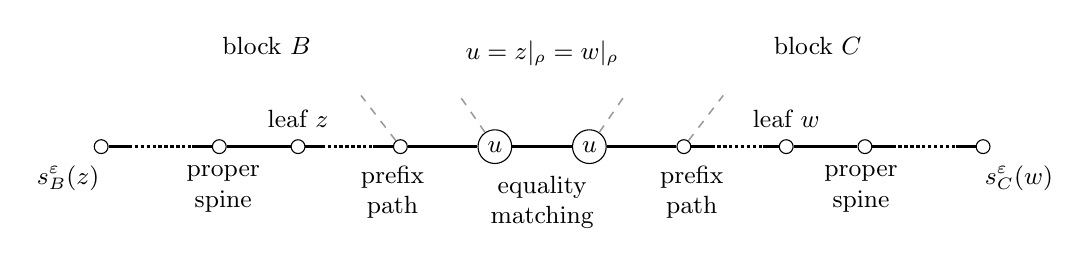
\begin{tikzpicture}[
  x=1cm,y=1cm,font=\small,
  vertex/.style={circle,draw,fill=white,inner sep=0pt,minimum size=5pt},
  root/.style={circle,draw,fill=white,inner sep=2pt},
  route/.style={line width=1.15pt},
  possible/.style={line width=.55pt,black!40,dashed}
]
  \node[vertex] (sB) at (-5.6,0) {};
  \node[vertex] (cB) at (-4.1,0) {};
  \node[vertex] (lB) at (-3.1,0) {};
  \node[vertex] (pB) at (-1.8,0) {};
  \node[root] (rB) at (-.6,0) {\(u\)};
  \node[root] (rC) at (.6,0) {\(u\)};
  \node[vertex] (pC) at (1.8,0) {};
  \node[vertex] (lC) at (3.1,0) {};
  \node[vertex] (cC) at (4.1,0) {};
  \node[vertex] (sC) at (5.6,0) {};
  \draw[route] (sB)--(-5.25,0) (-4.45,0)--(cB)--(lB);
  \draw[route,densely dotted] (-5.25,0)--(-4.45,0);
  \draw[route] (lB)--(-2.8,0) (-2.15,0)--(pB)--(rB);
  \draw[route,densely dotted] (-2.8,0)--(-2.15,0);
  \draw[route] (rB)--(rC)--(pC)--(2.15,0) (2.8,0)--(lC)--(cC);
  \draw[route,densely dotted] (2.15,0)--(2.8,0);
  \draw[route] (cC)--(4.45,0) (5.25,0)--(sC);
  \draw[route,densely dotted] (4.45,0)--(5.25,0);
  \draw[possible]
    (rB)--(-1.05,.65)
    (pB)--(-2.3,.65)
    (rC)--(1.05,.65)
    (pC)--(2.3,.65);
  \node[above] at (-3.5,1.05) {block \(B\)};
  \node[above] at (3.5,1.05) {block \(C\)};
  \node[below,anchor=north east] at (-5.5,-.12) {\(s_B^\eps(z)\)};
  \node[below,align=center] at (-4.05,-.12) {proper\\spine};
  \node[above] at (-3.1,.12) {leaf \(z\)};
  \node[below,align=center] at (-1.9,-.12) {prefix\\path};
  \node[below,align=center] at (1.9,-.12) {prefix\\path};
  \node[above] at (3.1,.12) {leaf \(w\)};
  \node[below,align=center] at (4.05,-.12) {proper\\spine};
  \node[below,anchor=north west] at (5.5,-.12) {\(s_C^\eps(w)\)};
  \node[below,align=center] at (0,-.25) {equality\\matching};
  \node[above] at (0,.9) {\(u=z|_\rho=w|_\rho\)};
\end{tikzpicture}
\caption{The walk that tests a shared readout \(\rho\).
The selected route follows a valuation's spine to the proper channel,
ascends its prefix tree to the root indexed by \(u\), crosses the
equality matching, and follows the opposite route to the other
distinguished vertex.
Dotted portions abbreviate intervening spine channels or tree levels.
Light dashed branches indicate possible additional legal prefixes;
the forests contain only prefixes with legal extensions and need not
be full binary trees.
A root and leaf coincide when their two levels agree.
Labels and line styles explain the diagram, without adding relations
to the colored graph.}
\label{graph:fig-readout-route}
\end{figure}


\Needspace{14\baselineskip}
\subsection{Translations that use one block offset}

\begin{lemma}[Colored block translations]
\label{graph:colored-translations}
Every \(\xi_B\in\cZ_B^1\) determines a color-preserving isomorphism
between the block parts of \(B\) in \(Y^0,Y^1\).
It fixes the anchor, sends
\[
 s_{Bc}^0(z)\longmapsto s_{Bc}^1(z+\xi_B),
 \qquad
 f_{Bc,h}^0(u)\longmapsto
 f_{Bc,h}^1\bigl(u+\pi_{Bc,h}(\xi_B)\bigr),
\]
and depends on no other block's offset.
On a union of parts, these maps form an induced-subgraph
isomorphism whenever the chosen offsets agree on shared names.
\end{lemma}

\begin{proof}
Translation by \(\xi_B\) bijects \(\cZ_B^0\) with \(\cZ_B^1\).
Its effect on a prefix depends only on that prefix and commutes with
truncation.  The displayed maps therefore give bijections at every
sort, preserving the tree, leaf-to-spine, and consecutive-channel
edges and their nonedges.
The empty prefix is fixed, so the anchor edge is preserved.

The only edges between parts are anchor-path edges and root-matching
edges.  Anchors are fixed individually.
For a root matching on \(\rho\), roots with values \(u,v\) are
adjacent exactly when \(u=v\).
If both block offsets have the same restriction \(d\) to \(\rho\),
then
\[
                       u=v\quad\Longleftrightarrow\quad u+d=v+d.
\]
This preserves both adjacency and nonadjacency across that matching.
Different channels stay different channels, so no other cross-part
adjacency can arise.
\end{proof}

\subsection{Removing the sort colors}

At each vertex \(v\) of \(Y^\eps\), assign its incident edges injectively
to ports \(1,2,3\), in any fixed construction order.
Replace \(v\) by a triangle with vertices
\[
                       t(v,1),\ t(v,2),\ t(v,3).
\]
For each \(j\), create a connector \(b(v,j)\) adjacent to \(t(v,j)\).
Attach a private path of length \(\operatorname{col}(v)\) to this
connector, with the connector as the path's initial vertex.
All other vertices on this path are new.
For an edge \(vw\) of \(Y^\eps\) assigned to ports \(j,j'\), add the
edge \(b(v,j)b(w,j')\).
No other edges or colors are retained.
Call the resulting uncolored graph \(X^\eps\).
The replacement gadget is shown in \Cref{graph:fig-uncoloring}.

Every new vertex made at \(v\) belongs to \(v\)'s block part.
In particular, the two endpoints of an edge between different blocks
belong to their respective blocks.
Denote these parts by \(V_B^\eps\).
The triangle replacing \(s_B^\eps(z)\) is denoted \(T_B^\eps(z)\).

\begin{figure}[tb]
\centering
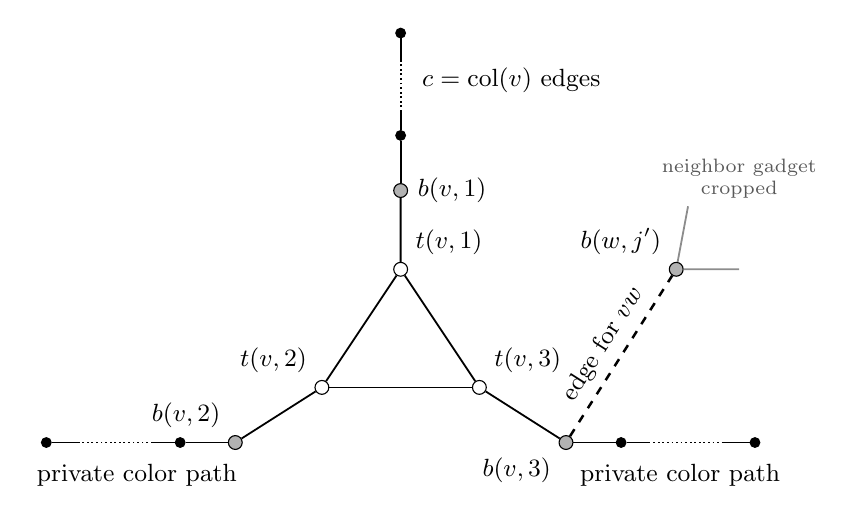
\begin{tikzpicture}[
  x=1cm,y=1cm,
  font=\small,
  vertex/.style={
    circle,draw,fill=white,inner sep=0pt,minimum size=5pt
  },
  connector/.style={vertex,fill=black!30},
  pathvertex/.style={vertex,fill=black,minimum size=3.5pt},
  graph edge/.style={line width=.65pt},
  external edge/.style={
    graph edge,dashed,line width=.9pt
  }
]
  \node[vertex,label=above right:{$t(v,1)$}] (t1) at (0,1) {};
  \node[vertex,label=above left:{$t(v,2)$}] (t2) at (-1,-.5) {};
  \node[vertex,label=above right:{$t(v,3)$}] (t3) at (1,-.5) {};
  \draw[graph edge] (t1)--(t2);
  \draw[graph edge] (t2)--(t3);
  \draw[graph edge] (t3)--(t1);
  \node[connector,label=right:{$b(v,1)$}] (b1) at (0,2) {};
  \node[connector,label=above left:{$b(v,2)$}]
    (b2) at (-2.1,-1.2) {};
  \node[connector,label=below left:{$b(v,3)$}]
    (b3) at (2.1,-1.2) {};
  \draw[graph edge] (t1)--(b1) (t2)--(b2) (t3)--(b3);

  \node[pathvertex] (p11) at (0,2.7) {};
  \node[pathvertex] (p1c) at (0,4) {};
  \draw[graph edge] (b1)--(p11)--(0,3);
  \draw[graph edge,densely dotted] (0,3)--(0,3.65);
  \draw[graph edge] (0,3.65)--(p1c);
  \node[right] at (.15,3.4)
    {$c=\operatorname{col}(v)$ edges};

  \node[pathvertex] (p21) at (-2.8,-1.2) {};
  \node[pathvertex] (p2c) at (-4.5,-1.2) {};
  \draw[graph edge] (b2)--(p21)--(-3.15,-1.2);
  \draw[graph edge,densely dotted]
    (-3.15,-1.2)--(-4.1,-1.2);
  \draw[graph edge] (-4.1,-1.2)--(p2c);
  \node[pathvertex] (p31) at (2.8,-1.2) {};
  \node[pathvertex] (p3c) at (4.5,-1.2) {};
  \draw[graph edge] (b3)--(p31)--(3.15,-1.2);
  \draw[graph edge,densely dotted]
    (3.15,-1.2)--(4.1,-1.2);
  \draw[graph edge] (4.1,-1.2)--(p3c);
  \node[below] at (-3.35,-1.35) {private color path};
  \node[below] at (3.55,-1.35) {private color path};

  \node[connector,label=above left:{$b(w,j')$}]
    (bw) at (3.5,1) {};
  \draw[external edge]
    (b3)--node[midway,above,sloped] {edge for \(vw\)} (bw);
  \draw[graph edge,black!45]
    (bw)--(3.65,1.8)
    (bw)--(4.3,1);
  \node[font=\scriptsize,black!65,align=center]
    at (4.3,2.15) {neighbor gadget\\cropped};
\end{tikzpicture}
\caption{The uncoloring gadget at a vertex \(v\).
Each triangle member has its own connector and each connector
has a private path of exactly \(c=\operatorname{col}(v)\) edges.
Dotted portions abbreviate path interiors; for \(c=1\), each private
path is a single pendant edge.
The dashed edge represents an original edge \(vw\) attached at its
chosen ports.  In this schematic example \(b(v,3)\) uses its external
port, while \(b(v,1)\) and \(b(v,2)\) do not.
The neighboring gadget is cropped, with its connector's other two
incidences shown as short stubs.
Shading and line styles explain the construction and are not graph
colors or additional relations.}
\label{graph:fig-uncoloring}
\end{figure}


\begin{lemma}[Uncolored promises and local lifts]
\label{graph:uncolored-lifts}
The graphs \(X^\eps\) are simple, connected, uncolored, and of maximum
degree at most three.  They have the same positive order, of size
\(O(N^4)\).
Each colored block translation in \Cref{graph:colored-translations}
has a fixed lift \(\Psi_{B,\xi_B}:V_B^0\to V_B^1\), depending only
on that offset, satisfying the induced-isomorphism assertion of
\Cref{prop:subcubic-realization}.
\end{lemma}

\begin{proof}
Every triangle member has degree three.
A connector has its triangle neighbor and its first path neighbor,
and, precisely when its port is used, one external connector neighbor.
Its degree is therefore two or three.
All other path vertices have degree at most two.
The edge lists introduce neither loops nor repeated edges.
Each replacement is connected, and replacements are joined exactly
along the original graph's edges; hence \(X^\eps\) is connected.
There is at least one block, each with nonempty legal valuations,
so the order is positive.

Fix a block and offset, and write \(v'\) for the image of a vertex
\(v\) under its colored block translation.
Define a permutation of the three ports at \(v\) to those at \(v'\)
as follows.
\begin{enumerate}
\item
A port used by an edge within the block goes to the port used by the
image of that edge under the colored translation.
\item
At an anchor, a port used by an external anchor-path edge goes to the
port for the anchor-path edge toward the same other block.
\item
At a proper-channel root, the port used by its edge to the opposite
root goes to the port for the unique such edge at its image root.
\item
The unused ports are matched in their fixed numerical orders.
\end{enumerate}
These prescriptions are disjoint and exhaustive.
Internal incidences are bijected by a within-block isomorphism.
Each anchor retains the same external anchor incidences, and each
proper root has exactly one external incidence at both source and
image.  Thus the unused port counts also agree, and the prescriptions
indeed give a permutation.
Crucially, the third prescription does not require the neighboring
block's offset.

Using this port permutation, map triangle members to triangle members,
connectors to connectors, and private paths in order to their
corresponding private paths.  The colors of \(v,v'\) agree, so the
path lengths agree.  This gives a bijection
\(\Psi_{B,\xi_B}\) of the block parts, with the asserted action on the
distinguished triangles.

For compatible offsets on a union of blocks, every internal edge and
every anchor edge is carried to the edge prescribed by its endpoint
port permutations.
For an equality matching, the root values are shifted by the same
readout offset, so the equality condition is preserved in both
directions.  At its two endpoints the unique external ports are
exactly the ports used by that matching.
Unused ports remain unused, and all channels remain their own channels.
It follows that all edges and nonedges between replacements in the
union are preserved.  The maps inside the replacements are also
isomorphisms, proving the induced-subgraph assertion.
Edges leaving the union impose no condition on unchosen offsets.

For equal orders, choose an arbitrary legal offset separately at each
block.  The resulting bijections of disjoint parts give a bijection
of the two vertex sets; compatibility is not needed for this count.
Finally, if the number of sorts is \(s\), a colored vertex of color
\(c\) produces exactly \(6+3c\) vertices.
By \Cref{graph:colored-promises}, both \(s\) and \(\abs{V(Y^\eps)}\)
are \(O(N^2)\), giving the order bound \(O(N^4)\).
All enumerations use at most six-bit valuations and prefixes, explicit
block pairs and shared names, and paths of polynomial length.
They therefore implement the construction in polynomial time.
\end{proof}

\subsection{What a winning game must preserve}

To establish the decoding hypothesis of \Cref{prop:game-reduction},
we use the reached-history principle from \Cref{game:section}.
A hypothetical continuation may discard unrelated pairs to test the
retained pairs. If failure of an asserted property would let Spoiler
force a loss, that property must already hold at the original history.
The test need not return to that history or restore discarded answers.
Thus the tests below establish invariants even when all slots are occupied.

\begin{lemma}[Recognition under a winning strategy]
\label{lem:graph-recognition}
Let \(K\ge6\), and fix a winning strategy on \(X^0,X^1\).
At every reached history:
\begin{enumerate}
\item
Paired vertices have the same degree and agree as to whether they lie
in a triangle.
\item
A triangle member over \(v\in V(Y^0)\) is paired with a triangle
member over some \(v'\in V(Y^1)\) of the same sort.
\item
If two marked triangle members lie over adjacent vertices \(v,w\)
of \(Y^0\), their responses lie over adjacent vertices \(v',w'\)
of \(Y^1\).
\item
A marked member of \(T_B^0(z)\) has a unique decoded response
\(z'\in\cZ_B^1\), meaning that its response belongs to \(T_B^1(z')\).
For simultaneous marked members at distinct blocks, equality of any
shared readout implies equality of the decoded response readouts.
\end{enumerate}
The conclusions do not require a free slot at the history in question.
\end{lemma}

\begin{proof}
\emph{Degrees and triangles.}
Retain a paired vertex and request one further slot.
For every vertex Spoiler could choose, Duplicator's announced
bijection must preserve adjacency to the retained vertex.
The bijection therefore takes its neighbor set onto the other
neighbor set, proving degree equality with two slots.
To test membership in a triangle, retain the vertex and mark the two
other triangle members, using three slots.
The converse can be tested in the second graph: after a bijection is
announced, Spoiler can choose the preimage of any desired
second-graph vertex.  Partial isomorphism then proves triangle
membership in both directions.

The only triangles in \(X^\eps\) are the designated replacement
triangles.
Indeed, private path vertices cannot lie in a triangle; a connector
has only one triangle-vertex neighbor; and edges between connectors
form a matching, since each connector is a single port.
There are no other edges between replacements.
Thus a response to a triangle member lies in a unique replacement
triangle.

\emph{Sort recovery.}
Retain such a pair, and mark the connector attached to its
first-graph triangle member.
By triangle membership and adjacency, its response is the unique
nontriangle neighbor of the second-graph triangle member.
At a connector, the first private-path vertex is its unique neighbor
of degree below three.
The triangle member has degree three, and any connector reached
across an external connector edge has degree three because that port
is used.  This assertion also covers an unused connector and a
private path of length one.
Consequently a third mark forces the first private-path step.

Continue along the source path, retaining the previous and current
vertices and using a third slot for the next vertex.
Adjacency and inequality from the previous vertex force the forward
step in the target private path.
The original triangle mark can be discarded once the traversal has
started.
If the lengths differed, at their first discrepancy a terminal vertex
of degree one would be paired with an internal vertex of degree two.
The degree invariant excludes this.
The path lengths, and therefore the sort numbers, are equal.
All assertions used during this test are invariants of reached
winning histories, established by their own alternative continuations.

\emph{Underlying adjacency.}
Retain the two marked triangle representatives over \(v,w\), and
also mark the actual triangle ports used by \(vw\) and the two
connectors attached to those ports.  This requires at most six slots.
An actual port may already be the representative; duplicate marking
is allowed, or its extra mark may be omitted.
Its response lies in the same triangle as its original
representative, by equality in the coincident case and by adjacency
and triangle membership otherwise.
Each connector response must be the unique nontriangle neighbor of
its port response.  The two connectors are adjacent, so their
underlying auxiliary vertices are adjacent in \(Y^1\).
The two response representatives cannot belong to one triangle:
the source representatives are distinct and nonadjacent, whereas
distinct members of one triangle are adjacent.

\emph{Distinguished vertices and shared readouts.}
Sort recovery sends a triangle over a channel-zero spine vertex
of block \(B\) to a triangle over another channel-zero spine vertex
of that same block.  The legal valuation indexing this vertex gives
the unique decoded response.

Suppose now that the two source valuations at distinct blocks agree
on a shared readout.
Their distinguished vertices admit the sort-prescribed walk from
\Cref{graph:readout-walk}.
First discard all marked pairs except these two endpoint pairs.
Mark triangle members over the intermediate vertices successively,
always retaining both endpoints and at most two consecutive
intermediate pairs.  Four slots suffice.
Sort recovery gives the required sorts of all response vertices.
Underlying adjacency, applied to each consecutive pair when both are
marked, shows that the responses trace a walk of precisely the
prescribed sorts.
\Cref{graph:readout-walk} now forces equality of the response readouts.

The four walk slots need not be supplemented by six adjacency-test
slots.  Underlying adjacency is already an invariant of every reached
winning history: its proof may discard the unrelated endpoint pairs
in a different continuation.  Similarly, the unary tests need not
retain the other walk marks.
The largest simultaneous test uses six slots, and the conclusion
about the retained endpoints therefore holds already at the original
history, regardless of its occupancy.
\end{proof}

\Needspace{8\baselineskip}
\begin{proof}[Proof of \Cref{prop:subcubic-realization}]
The graph promises, equal orders, size bound, local lifts, and
compatible-union isomorphisms are
\Cref{graph:colored-promises,graph:uncolored-lifts}.
The distinguished triangles have the stated indexing by construction.
Since \(K=r+1\ge9\), \Cref{lem:graph-recognition} supplies the
decoding and shared-readout invariants.
\end{proof}


\begin{corollary}[Correctness of the subcubic realization]
\label{cor:subcubic-game}
For every product scalar-image instance at address length \(r\ge8\),
its connected subcubic realization satisfies
\[
 \text{the instance is consistent}\quad\Longleftrightarrow\quad
 X^0\equiv_r X^1.
\]
\end{corollary}
\begin{proof}
Use \(\mathcal D_B^\eps(z)=T_B^\eps(z)\) in
\Cref{prop:game-reduction}. The block maps and decoding properties are
exactly those proved in \Cref{prop:subcubic-realization}; its parameter
condition holds because \(r\ge8\).
\end{proof}

\section{Uniform compilation and completeness}\label{uniform:section}

The algebraic witnesses are existential and are never supplied to the
graph compiler. We now enumerate only the product schemas, local blocks,
constant-size valuations, and graph vertices. The two realizations have
different output costs, so we retain their quantitative statements
separately. All operations are counted on deterministic multitape
Turing machines with sequential list access.

For the instance compiled from a fixed machine $M$ and polynomial $p$
as in \Cref{prop:computation}, on a word of length $m$, put
$r=2(p(m)+2)$ and $b_*=r+2$. Since $p(m)\ge m+2$, we have $m\le r$.
The common size calculation starts with $O_M(b_*^2)$ real types and
comparison schemas. Subdivision
multiplies this count by $O(r)$, and choosing a row for each local
block multiplies it by another $O(r)$. Thus there are $O_M(b_*^4)$
blocks, each with an absolute constant number of valuations.
The realizations then have the following growth:
\begin{center}
\begin{tabular}{@{}lll@{}}
\toprule
 & General realization & Subcubic realization\\
\midrule
Intermediate vertices & $O_M(b_*^4)$ base vertices
 & $O_M(b_*^8)$ auxiliary vertices\\
Block or sort encoding & $O_M(b_*^{12})$ vertices with leaves
 & $O_M(b_*^{16})$ vertices with color paths\\
Output matrix entries & $O_M(b_*^{24})$ & $O_M(b_*^{32})$\\
\bottomrule
\end{tabular}
\end{center}
The subcubic construction has $O_M(b_*^8)$ channels, with constantly
many auxiliary vertices per channel, and $O_M(b_*^8)$ sorts.
Replacing each auxiliary vertex by a gadget whose paths have length
at most the sort count gives the final $O_M(b_*^{16})$ order.
The proofs below justify these counts
and then account for the bit cost of producing the explicit matrices.
The constants may depend on the fixed $M,p$; the exponents in the
graph-size and compiler-time bounds are absolute.

\subsection{The smaller general compiler}

\begin{proposition}[Uniform general-graph compiler]\label{prop:uniform-general}
Fix the machine $M$ and polynomial $p$ used in
Proposition~\ref{prop:computation}. For a word $w$ of length $m$, put
$r=2(p(m)+2)$. The constructions of
\Cref{prop:computation,prop:consistency,prop:general-realization}
produce two equally large simple uncolored
graphs of order $O_M((r+1)^{12})$. Their explicit adjacency matrices and the
binary parameter $k=r$ can be produced by a deterministic multitape Turing
machine in time $O_{M,p}((r+2)^{80})$.
\end{proposition}
\begin{proof}
Since $p(m)\ge m+2$, we have $m\le r$. The number of original consistency
types and schemas is therefore $O_M((r+1)^2)$, and every vector dimension is
at most two. Each schema has $r$ constant-size binary coordinate entries.
Subdividing each wire with $4(r+1)$ internal types gives
$O_M((r+1)^3)$ types and links. Even copying an entire $r$-coordinate table
onto every link requires only $O_M((r+1)^4)$ entries.

For each type or link and each row there are at most four blocks: one chooses
two binary labels, or two label matches each determined by a binary label.
A site has at most four legal valuations. A square has two vector readouts
of dimensions at most two and two scalar readouts, hence at most $2^6$
valuations, a deliberately loose bound. Thus both the number $J$ of blocks
and the common number $N$ of base vertices are $O_M((r+1)^4)$; moreover
$J\le N$ because every block has a legal valuation in each version.
There are at most $J(N+1)$ leaves at any base vertex, giving total order
\begin{equation}\label{eq:graph-order-bound}
 N+NJ(N+1)\le N+N^2(N+1)=O_M((r+1)^{12}).
\end{equation}
The two output matrices have $O_M((r+1)^{24})$ entries in total.
There is at least one scalar real type, which alone supplies four sites per
row and two valuations per site. The graph order is at least $8r$, so the
output parameter is below the order.

Here is an explicit polynomial-time implementation. All lists are stored
sequentially, so no unit-cost random access is assumed.
\begin{enumerate}[label=\arabic*.,leftmargin=*]
\item Count $m$, evaluate the fixed polynomial $p$, and set $d,r,K$.
Enumerate the fixed machine alphabet, carry and borrow cases, initial
positions, and final-time tests. Fill each product table coordinate by
coordinate. Only the $\max\{1,m\}$ exceptional initial positions and the
$d+1$ possible blank suffix domains are generated. Apply the buffer and
dummy construction and enumerate wire and link identifiers.
\item Enumerate the constant number of local label choices for each
type-row or link-row pair. Record the named readouts of each block and
enumerate all of its local valuations. Test its affine or homogeneous
equation directly. Count $N$ and enumerate leaves by an owner identifier and
a local index. This produces vertex lists in both graph versions.
\item Enumerate ordered pairs of vertices and stream the corresponding
matrix bits. For base vertices, compare the constant number of named
readouts and their values, and check that the blocks differ. For a pair
involving a leaf, test owner incidence. Leaf--leaf pairs are nonadjacent.
The diagonal is zero. Finally write $r$ in binary.
\end{enumerate}

For a concrete bit-cost allowance, these descriptions use
$O_{M,p}((r+2)^{12})$ records, each of at most
$O_{M,p}((r+2)^2)$ bits; this includes full coordinate tables, identifiers,
valuation lists and counters. Allow the larger total work-space length
\[
 D=O_{M,p}((r+2)^{16}).
\]
The stated loops need at most $O_{M,p}((r+2)^{24})$ record-generation trials
and matrix entries. Each uses at most $O_{M,p}((r+2)^2)$ elementary lookups,
copies, comparisons or arithmetic operations; constructing a coordinate
table can scan all $r$ entries. A sequential list lookup or an elementary
binary arithmetic operation on at most $D$ bits costs $O(D^2)$ time by
ordinary scanning and schoolbook algorithms. The total allowance is thus
$O_{M,p}((r+2)^{24+2+32})$, which is within the asserted exponent~80.

Polynomial evaluation also fits this budget even if $p$ has signed
coefficients and cancellations. If $p(x)=\sum_{i=0}^q c_i x^i$ and
$A_p=1+\sum_i|c_i|$, every Horner intermediate at $m\ge0$ has absolute value
at most $A_p(m+1)^q$. Its bit length is $O_p(\log(r+2))$, and the number
$q$ of arithmetic stages is fixed. The case $m=0$ has $p(0)\ge2$ and causes
no exception. Reading the input and writing the $O(\log r)$-bit dimension
are included. At no stage is the list of $2^r$ full addresses, the
$2^d$ computation times, a consistency witness, or an offset family
enumerated.
\end{proof}


\subsection{The connected subcubic compiler}

\begin{proposition}[Uniform construction]
\label{prop:uniform-construction}
Fix a machine \(M\) and polynomial \(p\) satisfying
\Cref{prop:computation}, and apply the buffer construction
of \Cref{prop:consistency}.  On an input
word of length $m$, put
\[
 r=2(p(m)+2),\qquad K=r+1,\qquad b_*=r+2.
\]
The two graphs $X^0,X^1$ and the binary dimension $k=r$ can be produced
deterministically in time $O_{M,p}(b_*^{160})$.  Each output graph has
$O_M(b_*^{16})$ vertices.  They have the same positive order and are
connected, simple, uncolored, undirected graphs of maximum degree at most
three, regardless of whether the scalar-image instance is consistent.
\end{proposition}

\begin{proof}
We give explicit polynomial bounds and a construction that uses only the
compressed descriptions.  Since $p(m)\geq m+2$, we have $r\geq 8$ and
$m\leq b_*$.  The computation construction produces
$O_M((r+1)^2+m)=O_M(b_*^2)$ real types and comparison schemas.  Their
value dimensions are at most two.  A schema is described by its endpoint
identifiers, its two constant-size affine forms, and $r$ constant-size
coordinate domains and maps.

Each comparison wire has $4K$ private internal types and $4K+1$ links.
Thus the subdivided layout has $O_M(b_*^3)$ types and links.  At a fixed
row and type there are at most four choices of a site's pair of labels;
at a fixed row and link there are at most four choices of a square's two
coordinate matches.  Multiplying by $r$ rows gives
\begin{equation}
\label{uniform:block-bound}
 \abs{\cB}=O_M(b_*^4).
\end{equation}
A block has at most four readout names.  The total number of proper
channels, indexed by ordered pairs of distinct blocks and a shared name,
is therefore at most $4\abs{\cB}^2$.  Including channel zero at every
block, the total number of channels is $O_M(b_*^8)$.

Every legal valuation uses at most six bits by
\Cref{lem:block-fibers}.  Hence a channel has at most $2^6$ spine
vertices, at most seven prefix levels, and at most $2^6$ vertices on any
one of those levels.  These are absolute constants, independent of $r$.
There are also only constantly many vertex sorts per channel and one
anchor and anchor sort per block.  Consequently,
\begin{equation}
\label{uniform:auxiliary-bound}
 \abs{V(Y^\eps)}=O_M(b_*^8),\qquad
 s=O_M(b_*^8),
\end{equation}
where $s$ is the number of positive integer sort colors.

A colored vertex of color $c$ is replaced by three triangle vertices,
three connectors, and three private paths with $c$ new vertices each.
The replacement therefore has exactly $6+3c$ vertices.  Since
$1\leq c\leq s$, \eqref{uniform:auxiliary-bound} gives
\begin{equation}
\label{uniform:graph-bound}
 \abs{V(X^\eps)}
 \leq (6+3s)\abs{V(Y^\eps)}=O_M(b_*^{16}).
\end{equation}
The two explicit output matrices have $O_M(b_*^{32})$ entries, and the
output dimension $r$ has $O(\log b_*)$ binary bits.

All structural promises follow from \Cref{prop:subcubic-realization}.
In particular, equal order does not require a compatible global offset:
each individual block has a nonempty affine valuation space, and any of
its legal offsets supplies a bijection between its two block parts.
Their separate cardinalities agree and can be added over the partition.
There is at least one site block and a legal valuation in each version,
so the common graph order is positive.  Degree-one and degree-two vertices
are permitted because the required bound is at most three.

For completeness, the construction can be implemented with the following
finite lists and loops.
\begin{enumerate}
\item Evaluate the fixed polynomial $p$ and generate the circuit's schema
      domains and coordinate maps by the carry, borrow, and initialization
      cases of \Cref{prop:computation}.  Expand each connection into
      its comparison schemas, subdivide each comparison wire, and
      enumerate the type, link, and block lists.  A coordinate scan has
      length $r$; none of these steps ranges over the full set of
      addresses.
\item Compare the at most four names of each ordered pair of blocks to
      enumerate channels and their opposite-channel identifiers.  For
      every channel, enumerate bit strings of length at most six to list
      its legal valuations and occurring prefixes.  A prefix occurs if
      one of the constantly many full strings extending it satisfies the
      local equation.  Enumerate the sorts to assign their positive
      color numbers.  Fix all ordering choices by the same nested
      enumeration rules in the two versions.
\item Form the auxiliary vertex and edge lists from the defining rules.
      For example, enumerate unordered pairs of auxiliary vertices and
      test those rules.  Assign a vertex's incident ports in generated
      edge order; the list has length at most three.  Generate the
      triangle, connector, and private-path vertices using the sort
      numbers as path-length counters.
\item Enumerate pairs of output vertices and write their adjacency bits.
      A vertex record contains its original auxiliary vertex, its
      triangle/connector/path kind, its port, and, for a path vertex,
      its distance from the connector.  With the old edge and port lists,
      the replacement rules decide adjacency from such records.
\end{enumerate}
All local valuation tests have constant dimension.  The witness sets and
the families $\cH_U$ are used only in the correctness proof and are never
constructed by this algorithm.

Here is a deliberately loose bit-time accounting on a deterministic
multitape machine.  Individual records, coordinate tables, and counters
can be padded to $O_{M,p}(b_*^2)$ bits.  Identifiers and counters need only
$O_{M,p}(\log b_*)$ bits, and individual schema tables use $O(r)$ entries;
even a time or position address has only $d=r/2$ bits.  There are at most
$O_{M,p}(b_*^{32})$ records if the output matrix bits are included, so
$O_{M,p}(b_*^{40})$ bits suffice for lists and working storage, including
scratch space.  The fixed polynomial $p$ is evaluated on polynomially
bounded integers by ordinary integer arithmetic.

The ordered block-pair loop has $O_M(b_*^8)$ iterations, the auxiliary
vertex-pair loop has $O_M(b_*^{16})$, and the output pair loop has
$O_M(b_*^{32})$.  The other enumeration loops have no larger count.
The work of each iteration can be expressed using
$O_{M,p}(b_*^2)$ basic record operations: identifier lookup or update,
copying, comparison, and elementary integer arithmetic.  In particular,
edge information can be stored as endpoint and port records, without
copying whole adjacency rows into vertex records.  The total number of
these operations is bounded by $O_{M,p}(b_*^{40})$.

Implement an identifier lookup by a sequential scan of the stored lists;
all basic record operations can conservatively be bounded by the square
of the allowed tape length, using sequential scans and schoolbook
arithmetic.  Thus the preceding bounds give time at most
$O_{M,p}(b_*^{120})$, which is within the stated
$O_{M,p}(b_*^{160})$ allowance.  No constant or threshold in this
implementation depends on a separately fixed value of the growing
dimension.  Finally, $b_*$ is polynomial in $m$ for the fixed polynomial
$p$, so this is deterministic polynomial time in the source input length.
\end{proof}


\subsection{The two completeness reductions}

\begin{proof}[Proof of \Cref{thm:main}]
Membership for both languages is \Cref{prop:membership}, including
invalid encodings and dimensions larger than the graph order.

For hardness, fix any binary language \(L_0\in\EXPTIME\).
Choose a normalized deterministic decider \(M\) for its complement
and a fixed polynomial \(p\) as in \Cref{prop:computation-images}.
On \(w\) of length \(m\), generate the product circuit and its
scalar-image instance at \(r=2(p(m)+2)\ge8\). For \(\WL\), use
the general realization; for \(\SubWL\), use the connected subcubic
realization. Output the two explicit adjacency matrices and \(k=r\)
in binary. The compiler bounds are, respectively,
\(O_{M,p}((r+2)^{80})\) and \(O_{M,p}((r+2)^{160})\).
Since \(p\) is fixed, both are polynomial in \(m\); their polynomial
degrees may depend on the source language, as permitted for a
many-one reduction.

All required graph promises hold on every input, whether accepted
or rejected by \(M\). The two realization propositions verify the
hypotheses of \Cref{prop:game-reduction}. Together with the computation
reduction, this gives, for either output pair \(W^0,W^1\),
\[
\begin{aligned}
 w\in L_0
 &\Longleftrightarrow M\text{ does not accept }w\\
 &\Longleftrightarrow \text{the circuit has no true terminal test}\\
 &\Longleftrightarrow \text{the scalar-image instance is consistent}\\
 &\Longleftrightarrow W^0\equiv_r W^1.
\end{aligned}
\]
Thus each construction is a deterministic polynomial-time many-one
reduction with the required polarity. Because \(L_0\) was arbitrary,
both target languages are \(\EXPTIME\)-hard. No dimension-dependent
threshold or fixed-dimension lower bound supplies a step of these
uniform reductions.
\end{proof}


\begin{corollary}[Unary dimension]\label{cor:unary-dimension}
If the supplied dimension is encoded in unary instead of binary,
both \(\WL\) and \(\SubWL\) remain \(\EXPTIME\)-complete under
deterministic polynomial-time many-one reductions.
\end{corollary}

\begin{proof}
For membership, convert the unary dimension to binary and apply
\Cref{prop:membership}; the conversion is polynomial in the input length.
For hardness, the reductions just proved output
\(k=r=2(p(m)+2)\), which is polynomial in the source input length \(m\).
Writing this dimension in unary therefore preserves their polynomial
running time. The output graphs and the equivalence condition are
unchanged.
\end{proof}

\bibliographystyle{plainnat}
\bibliography{references}
\end{document}
